% **************************************************
% Document Class Definition
% **************************************************
\documentclass[%
    paper=A4,               % paper size --> A4 is default in Germany
    twoside=true,           % onesite or twoside printing
    openright,              % doublepage cleaning ends up right sidesirthe
    parskip=half,           % spacing value / method for paragraphs
    chapterprefix=true,     % prefix for chapter marks
    11pt,                   % font size
    headings=normal,        % size of headings
    bibliography=totoc,     % include bib in toc
    listof=totoc,           % include listof entries in toc
    titlepage=on,           % own page for each title page
    captions=tableabove,    % display table captions above the float env
    chapterprefix=false,    % do not display a prefix for chapters
    appendixprefix=false,    % but display a prefix for appendix chapter
    draft=false,            % value for draft version
]{scrreprt}%


% **************************************************
% Setup YOUR thesis document in this file !
% **************************************************
% !TEX root = my-thesis.tex


% **************************************************
% Files' Character Encoding
% **************************************************
\PassOptionsToPackage{utf8}{inputenc}
\usepackage{inputenc}


% **************************************************
% Information and Commands for Reuse
% **************************************************
\newcommand{\thesisTitle}{Sustaining glacial-fed catchments with artificial ice reservoirs}
\newcommand{\thesisName}{Suryanarayanan Balasubramanian}
\newcommand{\thesisSubject}{Artificial Ice Reservoirs}
\newcommand{\thesisDate}{\today}
\newcommand{\thesisVersion}{My First Draft}

\newcommand{\thesisFirstReviewer}{Felix Keller}
\newcommand{\thesisFirstReviewerUniversity}{\protect{ETH Zurich and Academia Engiadina}}
% \newcommand{\thesisFirstReviewerDepartment}{Department of Geosciences}

\newcommand{\thesisSecondReviewer}{Marcus Nüsser}
\newcommand{\thesisSecondReviewerUniversity}{\protect{South Asia Institute}}
% \newcommand{\thesisSecondReviewerDepartment}{Department of Clean Thesis Style}

\newcommand{\thesisThirdReviewer}{Michael Lehning}
\newcommand{\thesisThirdReviewerUniversity}{\protect{Swiss Federal Institute of Technology Lausanne and WSL Institute for Snow and Avalanche Research}}
% \newcommand{\thesisThirdReviewerDepartment}{Department of Clean Thesis Style}

\newcommand{\thesisFourthReviewer}{Thomas Vikhamar Schuler}
\newcommand{\thesisFourthReviewerUniversity}{\protect{University of Oslo}}
% \newcommand{\thesisFourthReviewerDepartment}{Department of Clean Thesis Style}

\newcommand{\thesisFirstSupervisor}{Martin Hoelzle}
% \newcommand{\thesisSecondSupervisor}{John Smith}

\newcommand{\thesisUniversity}{\protect{University Of Fribourg}}
\newcommand{\thesisUniversityDepartment}{Department of Geosciences}
\newcommand{\thesisUniversityInstitute}{Cryosphere Research Group}
\newcommand{\thesisUniversityGroup}{Cryosphere Research Group}
\newcommand{\thesisUniversityCity}{Fribourg}
\newcommand{\thesisUniversityStreetAddress}{Av. de l'Europe 20}
\newcommand{\thesisUniversityPostalCode}{CH-1700}


% **************************************************
% Debug LaTeX Information
% **************************************************
%\listfiles


% **************************************************
% Load and Configure Packages
% **************************************************
\usepackage[english]{babel} % babel system, adjust the language of the content
\PassOptionsToPackage{% setup clean thesis style
    figuresep=colon,%
    hangfigurecaption=false,%
    hangsection=true,%
    hangsubsection=true,%
    sansserif=false,%
    configurelistings=true,%
    colorize=bw,%
    colortheme=bluemagenta,%
    configurebiblatex=true,%
    bibsys=biber,%
    bibfile=zot_refs,%
    bibstyle=authoryear,%
    bibsorting=nty,%
}{cleanthesis}
\usepackage{cleanthesis}

\hypersetup{% setup the hyperref-package options
    pdftitle={\thesisTitle},    %   - title (PDF meta)
    pdfsubject={\thesisSubject},%   - subject (PDF meta)
    pdfauthor={\thesisName},    %   - author (PDF meta)
    plainpages=false,           %   -
    colorlinks=false,           %   - colorize links?
    pdfborder={0 0 0},          %   -
    breaklinks=true,            %   - allow line break inside links
    bookmarksnumbered=true,     %
    bookmarksopen=true          %
}

% **************************************************
% Other Packages
% **************************************************
\usepackage{scrhack}
\DeclareRobustCommand*\degree{\ensuremath{^{\circ}}}
\usepackage{siunitx} 
\usepackage{mathtools}
\usepackage{pdfpages}
\usepackage{booktabs}
\usepackage{acronym} 



% **************************************************
% Document CONTENT
% **************************************************
\begin{document}

% uncomment the following command to fill up pages with
% whitespace instead of aligning the first and last lines
% of a page (see \raggedbottom vs. \flushbottom)
%\raggedbottom

% --------------------------
% rename document parts
% --------------------------

% > set short label names for floating environments figure and table
%\renewcaptionname{ngerman}{\figurename}{Abb.}
%\renewcaptionname{ngerman}{\tablename}{Tab.}
\renewcaptionname{english}{\figurename}{Fig.}
\renewcaptionname{english}{\tablename}{Tab.}

% > rename the title of the LOL, i.e. list of listings (default is "Listings")
\renewcommand*{\lstlistlistingname}{List of abbreviations}

% --------------------------
% Front matter
% --------------------------
\pagenumbering{roman}			% roman page numbing (invisible for empty page style)
\pagestyle{empty}				% no header or footers
% !TEX root = ../my-thesis.tex
%
% ------------------------------------  --> cover title page
\begin{titlepage}
	\pdfbookmark[0]{Cover}{Cover}
	\flushright
	\hfill
	\vfill

  \begin{figure}[htb]
  \centering
  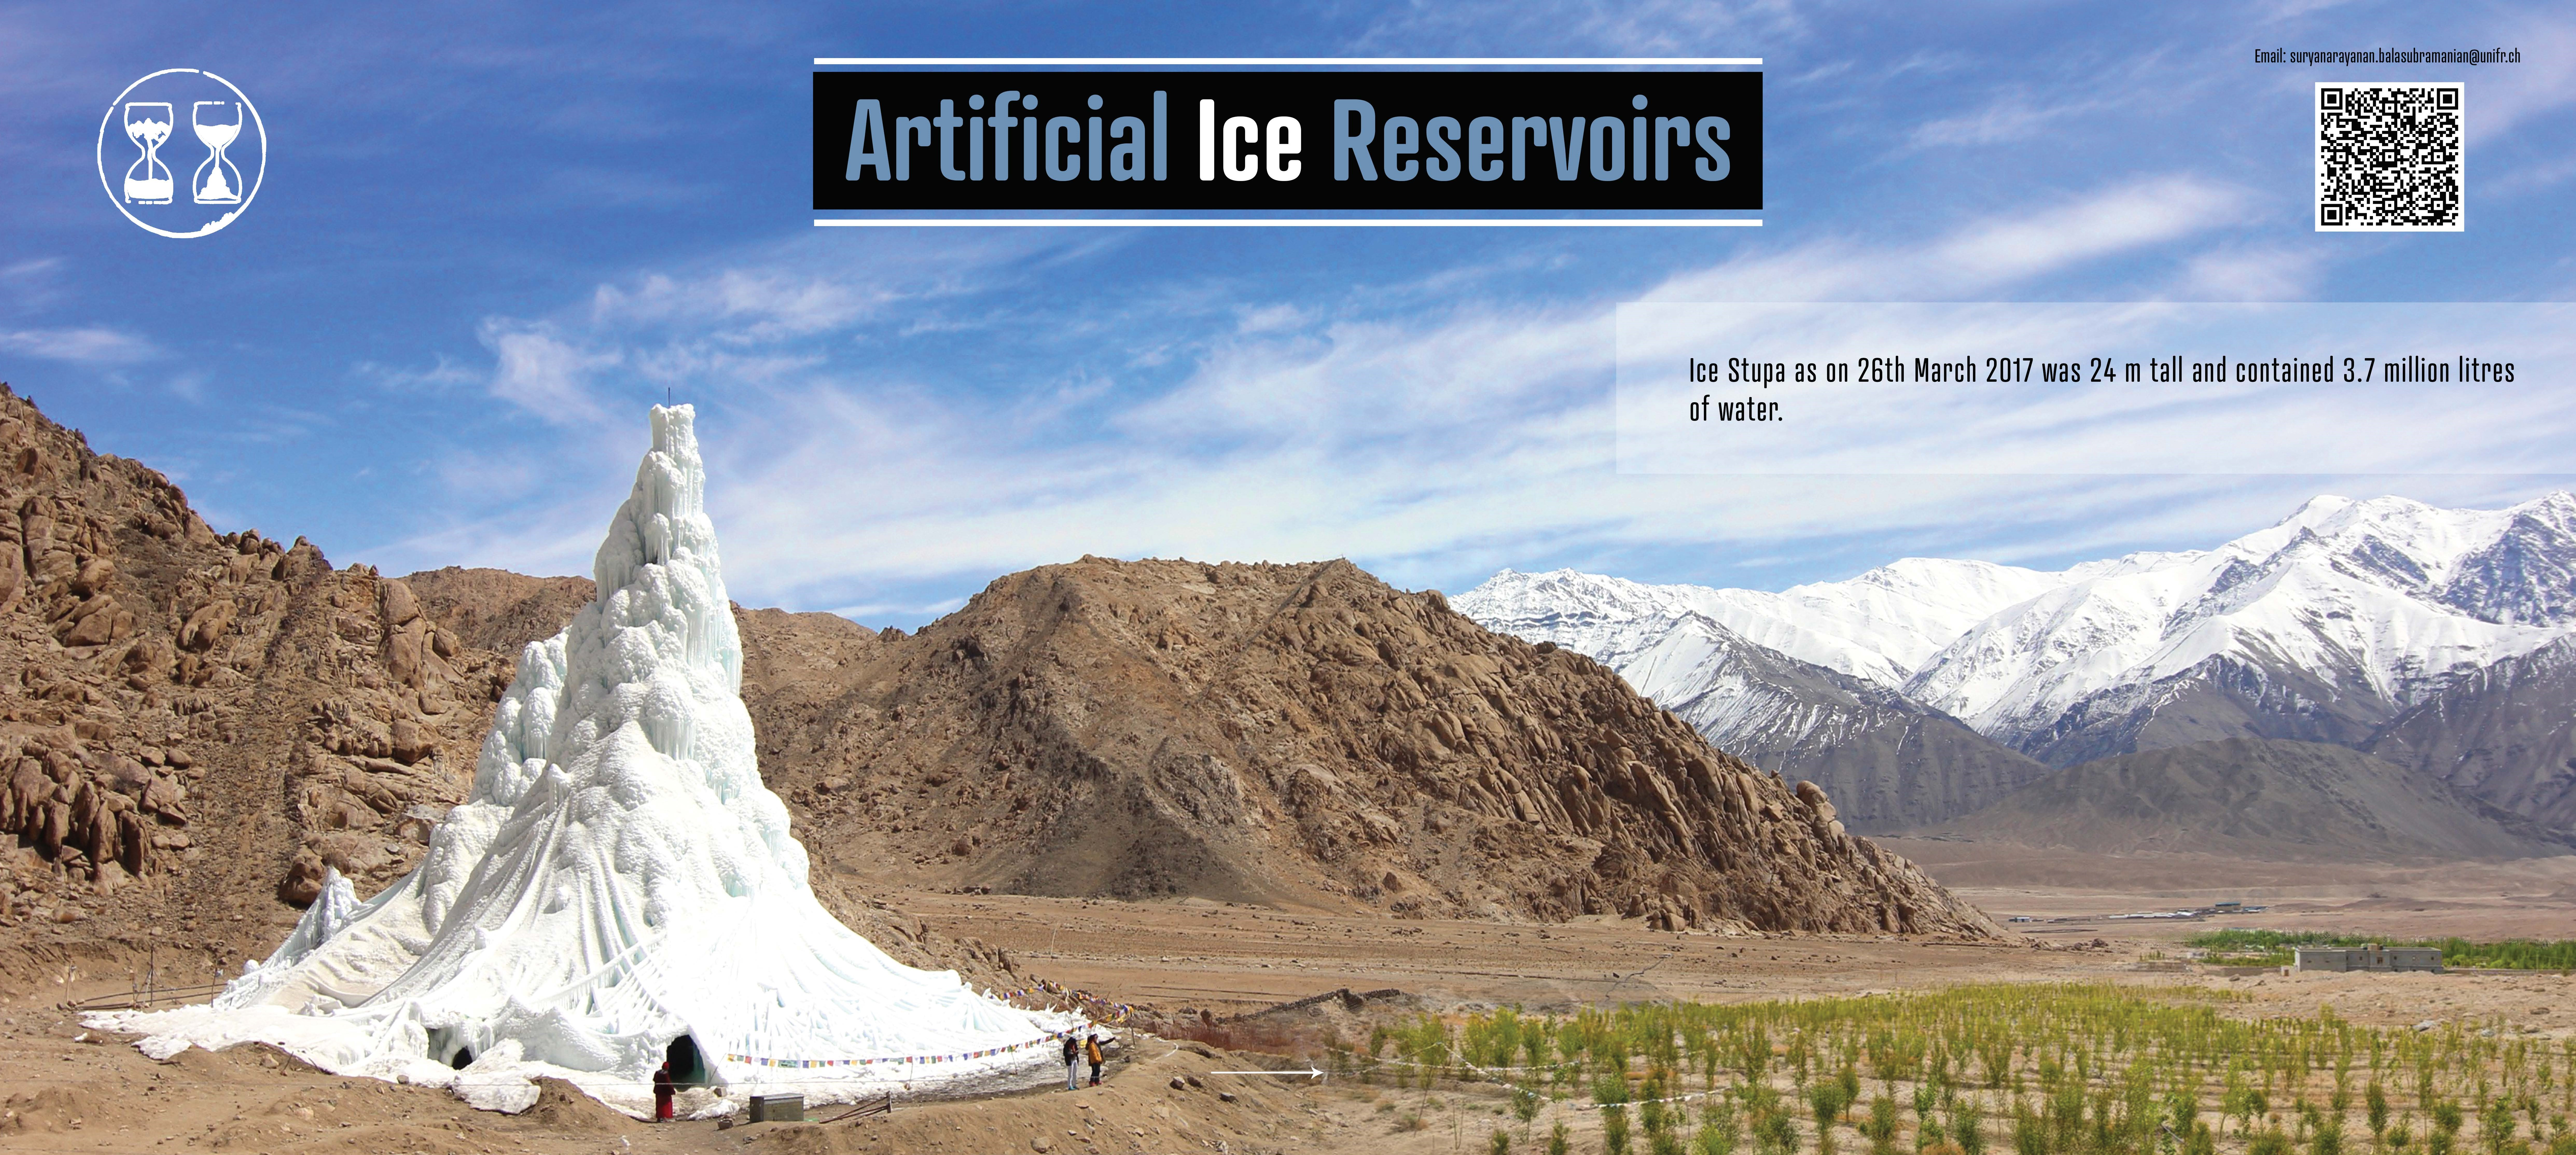
\includegraphics[width=\textwidth]{figs/AIR_title.jpg}
  \end{figure}
	{\Large\thesisTitle \par}
	\rule[5pt]{\textwidth}{.4pt} \par
	{\large\thesisName}
	\vfill
	\textit{\large\thesisDate} \\
	Version \thesisVersion
\end{titlepage}


% ------------------------------------  --> main title page
\begin{titlepage}
	\pdfbookmark[0]{Titlepage}{Titlepage}
	\tgherosfont
	\centering

	% {\Large \thesisUniversity} \\[4mm]
	\includegraphics[width=6cm]{figs/unifr-logo} \\[2mm]
	\textsf{\thesisUniversityDepartment} \\
	% \textsf{\thesisUniversityInstitute} \\
	\textsf{\thesisUniversityGroup} \\

	\vfill
	\includegraphics[width=3cm]{figs/air_logo_circle} \\[2mm]
	% {\large \thesisSubject} \\[5mm]
	{\LARGE \color{ctcolortitle}\textbf{\thesisTitle} \\[10mm]}
	{\Large \thesisName} \\

	\vfill
	% \begin{minipage}[t]{.27\textwidth}
	% 	\raggedleft
	% 	\textit{1. Reviewer}
	% \end{minipage}
	% \hspace*{15pt}
	% \begin{minipage}[t]{.65\textwidth}
	% 	{\Large \thesisFirstReviewer} \\
	%   	% {\small \thesisFirstReviewerDepartment} \\[-1mm]
	% 	{\small \thesisFirstReviewerUniversity}
	% \end{minipage} \\[5mm]
	% \begin{minipage}[t]{.27\textwidth}
	% 	\raggedleft
	% 	\textit{2. Reviewer}
	% \end{minipage}
	% \hspace*{15pt}
	% \begin{minipage}[t]{.65\textwidth}
	% 	{\Large \thesisSecondReviewer} \\
	%   	% {\small \thesisSecondReviewerDepartment} \\[-1mm]
	% 	{\small \thesisSecondReviewerUniversity}
	% \end{minipage} \\[10mm]
	% \begin{minipage}[t]{.27\textwidth}
	% 	\raggedleft
	% 	\textit{3. Reviewer}
	% \end{minipage}
	% \hspace*{15pt}
	% \begin{minipage}[t]{.65\textwidth}
	% 	{\Large \thesisThirdReviewer} \\
	%   	% {\small \thesisThirdReviewerDepartment} \\[-1mm]
	% 	{\small \thesisThirdReviewerUniversity}
	% \end{minipage} \\[10mm]
	% \begin{minipage}[t]{.27\textwidth}
	% 	\raggedleft
	% 	\textit{4. Reviewer}
	% \end{minipage}
	% \hspace*{15pt}
	% \begin{minipage}[t]{.65\textwidth}
	% 	{\Large \thesisFourthReviewer} \\
	%   	% {\small \thesisFourthReviewerDepartment} \\[-1mm]
	% 	{\small \thesisFourthReviewerUniversity}
	% \end{minipage} \\[10mm]
	% \begin{minipage}[t]{.27\textwidth}
	% 	\raggedleft
	% 	\textit{Supervisor}
	% \end{minipage}
	% \hspace*{15pt}
	% \begin{minipage}[t]{.65\textwidth}
	% 	\thesisFirstSupervisor\
	% \end{minipage} \\[10mm]
	\begin{minipage}[t]{.27\textwidth}
		\raggedleft
		\textit{Supervisor}
	\end{minipage}
	\hspace*{15pt}
	\begin{minipage}[t]{.65\textwidth}
		{\Large \thesisFirstSupervisor} \\
	\end{minipage} \\[10mm]

	\thesisDate \\

\end{titlepage}


% ------------------------------------  --> lower title back for single page layout

This thesis was presented to the Faculty of Science of the University of Fribourg (Switzerland) in consideration
for the award of \textit{Doctor rerum naturalium} on \thesisDate.

\vfill
{\large \textbf{Citation} \\}
Balasubramanian, S. \thesisTitle . \thesisUniversityGroup, 2022.

\hfill
\vfill
{
	\small
	\textbf{\thesisName} \\
	\textit{\thesisTitle} \\
	\thesisSubject, \thesisDate \\
	Reviewers: \thesisFirstReviewer,\ \thesisSecondReviewer,\ \thesisThirdReviewer\ and \thesisFourthReviewer \\
	Supervisor: \thesisFirstSupervisor \\
	English editors: Lou Del Bello\ and Ana Rodríguez Crespo\\[1.5em]
	\textbf{\thesisUniversity} \\
	\textit{\thesisUniversityGroup} \\
	% \thesisUniversityInstitute \\
	\thesisUniversityDepartment \\
	\thesisUniversityStreetAddress \\
	\thesisUniversityCity \\
	\thesisUniversityPostalCode \\
  \url{https://www.unifr.ch/geo/cryosphere/en/}\\
\\
  This thesis was typeset with \LaTeXe.
  It uses the \textit{Clean Thesis} style developed by Ricardo Langner.
  Download the \textit{Clean Thesis} style at \url{http://cleanthesis.der-ric.de/}.
}

		% INCLUDE: all titlepages
\cleardoublepage
%
% % !TEX root = ../my-thesis.tex
%
\pagestyle{plain}
\pdfbookmark[0]{Preface}{Preface}
\addchap{Preface}

Please put your preface here.

\bigskip

\noindent\textit{\thesisUniversityCity, \thesisDate}

\smallskip

\begin{flushright}
	\begin{minipage}{5cm}
		\rule{\textwidth}{1pt}
		\centering\thesisFirstSupervisor
	\end{minipage}
\end{flushright}

%*****************************************
%*****************************************
 
% \cleardoublepage
%

\pagestyle{plain}				% display just page numbers
% \pdfbookmark[0]{Summary}{Summary}
\addchap{Summary}
\label{sec:summary}

Irrigated agriculture is crucial for the livelihood security of mountain communities. Using meltwater from
glaciers, snow and permafrost, mountain dwellers have developed sophisticated techniques to cope with recurrent
water scarcity caused by glacial retreat and seasonal snow-cover dynamics. Artificial ice reservoirs (AIRs) are
a key example of community-based water management. Worldwide, farmers in around 30 mountain villages build these
ice structures. These seasonal ice reservoirs increase meltwater availability during the critical period of
water scarcity. To assess the role of AIRs within the water resource management of mountain villages under a
changing climate, they need to be represented in integrated modelling frameworks. Efficient water storage can be
achieved by taking into account their local meteorological conditions and water availability throughout the
year. This thesis aims to increase the understanding of volume dynamics of AIRs to provide tools to reduce their
water losses and maintenance requirements.

The different contributions of surface processes of the AIRs built in Guttannen, Switzerland and  Gangles, India
were estimated. These two locations present different meteorological patterns due to their significant
latitudinal and altitudinal differences. Using AIR-specific mass and energy balance models that consider
meteorological factors, fountain discharge, and ice volume changes, surface processes were quantified and
compared across the two locations. The models successfully estimated the observed ice volume evolution with a
root mean square error within 20\% of the maximum ice volume for five AIRs. The location in Ladakh presented a
maximum ice volume four times larger than that of the Guttannen site. However, poor fountain operation resulted
in wastage of more than four fifths of the provided water supply. These results highlight the relevance of
colder drier climates and fountain water supply management in the optimization of AIR construction.

In addition, AIR water loss reduction was attempted on the Swiss Alps by implementing fountain scheduling
strategies. Fountain scheduling was performed using a ball valve automated with optimal discharge rates computed
using AIR models. Simulations converting nonscheduled fountains into scheduled fountains showed a more than
threefold improvement in the water use efficiency of several AIRs. Fountain operation using scheduling
strategies produced similar ice volumes while consuming one tenth of the water compared with their nonscheduled
counterparts. Overall, these results show that automated fountain water supply management can both increase the
water-use efficiency of AIRs and reduce their maintenance needs without compromising their meltwater production.

This thesis introduces, for the first time, a model- and measurement-based understanding on the volume evolution
of AIRs under different climates; it also presents methods to quantify the storage potential of these ice
structures worldwide and practical tools to improve their efficacy. This study improves the scientific evidence
needed to upscale this indigenous water storage technology. These findings are essential to design these
nature-based solutions that increase the reliability of water supply in highly seasonal and arid environments
and improve water security and climate change adaptation in mountain regions. Future work may build on this
research by fully integrating climate change scenarios to investigate the potential hydrological contributions
of ice harvesting technologies for water-stressed mountain catchments.

\addchap{Résumé}

L'agriculture irriguée est cruciale pour sécuriser les moyens de subsistance des communautés de montagne. En utilisant les eaux issues de la fonte des glaciers, de la neige et du pergélisol, les habitants des montagnes ont développé des techniques sophistiquées pour faire face à la pénurie d'eau récurrente causée par le retrait des glaciers et la variabilité saisonnière de la couverture neigeuse. Les réservoirs de glace artificiels (RIA) sont un exemple clé de gestion communautaire de l'eau. Dans le monde entier, les agriculteurs d'une trentaine de villages de montagne construisent ces structures de glace. Ces réservoirs de glace saisonniers augmentent la quantité d’eau de fonte disponible pendant la période critique de pénurie d'eau. Pour évaluer le rôle des RIA au sein de la gestion des ressources en eau des villages de montagne dans un contexte de changement climatique, il est nécessaire de les représenter dans des cadres de modélisation intégrés. En tenant compte des conditions météorologiques locales et de la disponibilité de l'eau tout au long de l'année, l'eau peut être efficacement stockée. Cette thèse vise à améliorer la compréhension de la dynamique des volumes des RIA afin de fournir des outils pour réduire leurs pertes d'eau et besoins d'entretien. 

Les différentes contributions des processus de surface ont été estimées pour des RIA construits à Guttannen, en Suisse, et à Gangles, au Ladakh en Inde. Ces deux sites sont affectés par des conditions météorologiques distinctes en raison de leurs importantes différences latitudinales et altitudinales. À l'aide de modèles de bilan de masse et d'énergie spécifiques aux RIAs qui prennent en compte les facteurs météorologiques, le débit des fontaines et les changements de volume de glace, les processus de surface ont été quantifiés et comparés entre les deux sites. Les modèles ont reproduit avec succès l'évolution observée du volume de glace de cinq RIA avec une erreur quadratique moyenne de 20 \% du volume maximal de glace. Le site du Ladakh présentait un volume maximal de glace quatre fois supérieur à celui du site de Guttannen. Cependant, le mauvais fonctionnement de la fontaine a entraîné un gaspillage de plus de quatre cinquièmes de la quantité d'eau disponible. Ces résultats soulignent l'importance des climats plus froids et plus secs et de la gestion de l'approvisionnement en eau des fontaines dans l'optimisation de la construction des RIAs. 

En outre, grâce à différentes stratégies de programmation des fontaines, des essais de réduction des pertes d'eau ont été effectué dans les Alpes suisses. La programmation des fontaines a été réalisée à l'aide d'une vanne à bille automatisée permettant l’ajustement du débit aux valeurs optimales calculées à l'aide des modèles de RIA. Des simulations comparant des fontaines non programmées avec des fontaines programmées ont montré une amélioration de plus de trois fois de l'efficacité de l'utilisation de l'eau de plusieurs RIAs. Le fonctionnement des fontaines utilisant des stratégies de programmation a produit des volumes de glace similaires tout en consommant un dixième de la quantité d’eau de leurs homologues non programmées. Dans l'ensemble, ces résultats montrent que la gestion automatisée de l'approvisionnement en eau des fontaines peut à la fois augmenter l'efficacité de l'utilisation de l'eau des RIAs et réduire leurs besoins de maintenance sans compromettre leur production d'eau de fonte.

Cette thèse présente, pour la première fois, une compréhension de l'évolution du volume des RIAs sous différents climats sur la base de modèles et de mesures; elle présente également des méthodes pour quantifier le potentiel de stockage de ces structures de glace dans le monde entier et des outils pratiques pour améliorer leur efficacité. Cette étude améliore les connaissances scientifiques nécessaires à l'expansion de cette technologie indigène de stockage de l'eau. Ces résultats sont essentiels à la conception de solutions naturelles augmentant la fiabilité de l'approvisionnement en eau dans les environnements arides dépendant de source d’eau saisonnières. Ils contribuent à l’amélioration de la sécurité de l’approvisionnement en eau et à l'adaptation au changement climatique des régions de montagnes. De futurs travaux pourraient s'appuyer sur cette recherche en intégrant pleinement les scénarios de changement climatique afin d’étudier les potentielles contributions hydrologiques de ces technologies de récolte de la glace au niveau des bassins versants soumis à un stress hydrique.		% INCLUDE: the abstracts (english and german)
\cleardoublepage

\currentpdfbookmark{\contentsname}{toc}
\setcounter{tocdepth}{2}		% define depth of toc
\tableofcontents				% display table of contents
\cleardoublepage

% --------------------------
% Body matter
% --------------------------
\pagenumbering{arabic}			% arabic page numbering
\setcounter{page}{1}			% set page counter
\pagestyle{scrheadings}			% header and footer style

%% Uncomment the following lines using the \part command
%% to add part sections
\chapter{Ice Reservoirs}

\cleanchapterquote{Glaciers are the secret of life in these otherwise lifeless deserts. But now, they are
melting away at an alarming rate.}{Sonam Wangchuk}{(Ramon Magsaysay awardee, Inventor of ice stupas)}

\section{Introduction}

Cryosphere-fed irrigation networks in arid mountain regions are completely dependent on the timely availability
of meltwater from glaciers, snow and permafrost \citep{immerzeelImportanceVulnerabilityWorld2020,
farhanHydrologicalRegimesConjunction2015, tveitenGlacierGrowingLocal2007}. With the accelerated decline of
glaciers due to climate change \citep{nusserLocalKnowledgeGlobal2016}, these regions are experiencing water
scarcity \citep{norphelSnowWaterHarvesting2015, mukhopadhyayReevaluationSnowmeltGlacial2015}. Further, the
unreliability and the foreseen decrease of seasonal snow cover \citep{chevuturiClimateChangeLeh2018} increase
the precariousness of the water storage function of the cryosphere, especially in spring.

For example, due to the short growing period, central Ladakh is a single-cropping area with barley and wheat as
important staples, complemented by vegetables, pulses, and oil seeds
\citep{nusserSociohydrologyArtificialGlaciers2019}. Depending on altitudinal position, irrigation with complete
flooding of fields (approximately 2-5 cm water column) starts between March and April prior to the melting of
high-altitude glaciers ( Fig. \ref{fig:irrigation_cycles}). This results in increased demand during a period of
reduced supply at the onset of the agricultural season ( Fig. \ref{fig:irrigation_cycles}).

\begin{figure}[htb]
\centering
\includegraphics[width=\textwidth]{figs/irrigation_cycles.png}
\caption{Seasonal variation in the availability of irrigation water. The graph highlights the crucial role of
AIRs in bridging the critical gap in water availability. Adapted from \cite{nusserLocalKnowledgeGlobal2016}}
\label{fig:irrigation_cycles}
\end{figure}

To cope with this recurrent water scarcity, villagers have developed two types of artificial ice reservoirs
(AIRs): ice stupas and ice terraces ( Fig. \ref{fig:AIRforms}). Both the ice reservoirs capture water in the
autumn and winter, allowing it to freeze, and hold it until spring, when it melts and flows down to the fields
\citep{ipccChapterHighMountain2019, vinceGlacierMan2009, clouseLadakhArtificialGlaciers2017,
nusserSociohydrologyArtificialGlaciers2019}. In this way, they retain a previously unused portion of the annual
flow and facilitate its use to supplement the decreased flow in the next spring ( Fig.
\ref{fig:irrigation_cycles}).

\begin{figure}[t]
\centering
\includegraphics[width=\textwidth]{figs/AIR_forms.jpg}

\caption{(a) Schematic overview of the position of artificial ice reservoirs. These constructions are located at
  altitudes between the glaciers and the irrigation networks in the cultivated areas. (b) Ice terraces at 3900
  m, located above the village of Nang, Ladakh. The cascade is composed of a series of loose masonry walls
  ranging in height from 2 to 3 $m$, which help freeze water for storage. (c) Ice stupas at 3600 m, located
above the village of Phyang, Ladakh. They are made using fountain systems. Adapted from
\cite{nusserLocalKnowledgeGlobal2016}}

\label{fig:AIRforms}
\end{figure}

There is a long tradition of developing such ice harvesting structures in the upper Indus Basin, in both Ladakh,
northern India \citep{labbalTraditionalOasesLadakh2000, nusserIrrigationDevelopmentUpper2012} and various
locations in northern Pakistan \citep{kreutzmannScarcityOpulenceWater2011}. According to oral history and Corona
imagery from 1969, the first ice terraces are older than 50 years. Over the past decade, several ice stupas have been built to supplement the irrigation water supply of mountain
villages in India \citep{wangchukIceStupaCompetition2020, palmerStoringFrozenWater2022,
aggarwalAdaptationClimateChange2021}, Kyrgyzstan \citep{bbcnewsBrightArtificialGlacier2020}, and Chile
\citep{reutersConservationistsChileAim2021}.


Despite this widespread adoption, only a few publications examine the role of AIRs in the water resource
management in these regions. Notably, none of these prior reports have investigated AIRs outside Ladakh.
Moreover, quantifications of water storage capacity of AIRs in Ladakh vary widely between these studies
\citep{norphelSnowWaterHarvesting2015, baglaArtificialGlaciersHelp1998}.

Quantifying the water storage capacity of AIRs is not straightforward since the processes by which AIRs are
formed are complex. These processes are controlled by local topography, meteorology and the construction
strategies used. Modelling approaches to quantify these processes exist on glacier surfaces but they are not
readily applicable for AIRs due to their limited size, and comparatively more variable surface area. Therefore,
further modification of glacial modelling approaches are required for them to be sensitive to the
spatio-temporal scale of AIR surface processes. Furthermore, these modelling approaches need to be validated and
calibrated with comprehensive data from in-situ field measurements. 

A spirit of improvisation guides the construction strategies of AIRs \citep{clouseLadakhArtificialGlaciers2017}.
Depending on the topography of the construction location and how water is supplied, AIRs can form as flat sheets
or vertical cones. This has resulted in ice reservoirs exhibiting significant volume variations despite
experiencing similar meteorological conditions. For example, ice terraces have attained volumes upto 30 times
larger than ice stupas built in Ladakh, India \citep{nusserSociohydrologyArtificialGlaciers2019}. However, the
processes driving these differences can only be understood if the complete methodology behind the construction
strategy used is available.

This thesis aims to fulfill both of these requirements by providing a new set of AIR-specific volume and area
measurements via drone flights, along with meteorological data during the construction period. All these
datasets were generated through construction strategies that used fountain systems. These systems are quantified via in-situ
observations of the fountain characteristics and discharge rate measurements. First, this thesis
formulates a one-dimensional AIR model in order to calibrate and validate it with the procured AIR datasets.
Second, the thesis uses this model as a tool to propose a construction strategy that can produce AIRs
efficiently and effortlessly. It is important to note that while this thesis reviews published AIR research and
presents a comprehensive quantitative study of their water storage potential, we acknowledge that the farming
communities building these structures since mid-1800s hold substantial additional knowledge.


\section{Nomenclature and Classification}

While the term "artificial glacier" is more commonly used, we deliberately use the term "ice reservoir" in this
thesis. By definition, all glaciers, including the smallest ones, are bodies of sedimentary ice which were built
up by progressive snow compaction and firnification and flow downhill under the influence of gravity
\citep{benndouglasiGlaciersGlaciation2014}. Hence, because of their genesis and composition, AIRs differ from
glaciers. Man-made ice structures typically have a lifetime in the order of months and a size million times
smaller than typical glaciers. Therefore, any comparison between these ice structures can be misleading. Since
glaciers are considered as natural ice reservoirs, we use the terminology artificial ice reservoirs (AIRs) to
distinguish the man-made ice structures described in this thesis from the natural ones. 

% This is because it conveys the character and function of these structures more accurately
% \citep{nusserSociohydrologyArtificialGlaciers2019}. 

However, when classified in terms of size and survival duration, AIRs exhibit similar characterestics to
very small glaciers. The glossary of glacier mass balance and related terms by
\citet{cogleyGlossaryGlacierMass2010} defines very small glaciers or glacierets as follows:

\begin{thesis_quotation}
  A very small glacier, typically less than 0.25 $km^2$ in extent, with no marked flow pattern
  visible at the surface. To qualify as a glacieret, an ice body must persist for at least two consecutive
  years. Glacierets can be of any shape, and usually occupy sheltered parts of the landscape. Windborne snow and
  avalanches can be dominant contributors to the accumulation of glacierets.
\end{thesis_quotation}

This rather broad definition of glacierets or very small glaciers may be the one best suited for AIRs since
they have been measured with areas as high as 0.15 $km^2$ and observed to last beyond a year.

As has been noted above, a spirit of improvisation guides the construction strategy of AIRs challenging their
classification. However, it has been found that construction strategies that use fountain systems form conical
AIRs, while those that don't form flat sheets of ice. Therefore, this thesis classifies all the AIRs produced
based on whether or not they use fountain systems. AIRs using fountain systems are called "ice stupas" and those
without are called "ice terraces" as this terminology denotes the resulting shape of the respective AIRs
appropriately.

\section{Objectives}

We applied an integrated approach for this study, including field measurements and modelling, to answer the
following research questions: 

\begin{enumerate}

\item What is the influence of construction location and fountain characteristics on AIR volume evolution? 

\item How can ice stupa fountain systems be engineered to reduce water loss and maintenance efforts of AIRs?

\end{enumerate}

An energy and mass balance model for artificial ice reservoirs was set up to answer the first research question
(paper I and III). Since in-situ measurements were required to run this model, we executed a measurement campaign
in Switzerland and India during the past 4 winters. These datasets provided the necessary input, calibration and
validation data to model the evolution of AIRs and study their sensitivity to meteorological conditions and
fountain characteristics (paper II). 

We also developed new construction strategies to answer the second research question. These construction
strategies employed fountains whose discharge rate was regulated by an automation system that used the AIR model
developed before. Their advantages over traditional construction strategies are quantified in paper II.

\section{Structure}

Chapter 1 introduces the motivation of this work and provides a summary of the state of knowledge about AIRs
prior to this thesis. Chapter 2 describes the origins of this technology as a religious practice. Chapter 3
gives an overview about the study sites and introduces the different field techniques applied. The engineering
design of AIR technologies are showcased in Chapter 4 along with suggestions for their improvement. The observed
spatio-temporal variations in AIR volume evolution are presented in Chapter 5 along with suggestions for
choosing future construction locations. Chapter 6 concludes the thesis with a synthesis and the future scope of
this work. Papers I, II and III are included in the Appendix.

% Over the past 30 years, 14 ice terraces have
% been constructed in central Ladakh, located in tributary valleys of the Indus
% \citep{norphelArtificialGlacierHigh2009, nusserSociohydrologyArtificialGlaciers2019}. Chewang Norphel, a well
% known engineer of the Leh Nutrition Project, introduced this practice to Ladakh \citep{vinceGlacierMan2009}.

% Ice stupas were invented by Sonam Wangchuk in 2013 \citep{wangchukIceStupaArtificial2014} to provide a much
% cheaper alternative to achieve water storage compared to ice terraces. Ice stupas can also be placed much closer
% to the plantations since they absorb lesser solar radiation per unit volume compared to ice terraces due to
% their conical shape. However, the typical volume range of ice stupas ( Fig. \ref{fig:airs_ladakh}) are also
% much smaller than ice terraces. Over the past decade, several ice stupas have been built to supplement
% irrigation water supply of mountain villages in India \citep{wangchukIceStupaCompetition2020,
% palmerStoringFrozenWater2022, aggarwalAdaptationClimateChange2021}, Kyrgyzstan
% \citep{bbcnewsBrightArtificialGlacier2020} and Chile \citep{reutersConservationistsChileAim2021}.
   % INCLUDE: introduction
\chapter{Religion of ice reservoirs}

\cleanchapterquote{We believe that glaciers are alive. That's why a combination of
female and male ice was necessary.}{Liaquat Ali Baltee}{(Resident of Skardu, Pakistan)}

For centuries, in the Himalayan mountain ranges, local cultures have believed that glaciers are alive and that
certain glaciers can also have different genders. These local communities ‘breed’ new glaciers by grafting
together —or marrying— fragments of ice from male and female glaciers covering them with charcoal, wheat husks,
cloths, or willow branches so they can reproduce in privacy. These glacierets transform into fully active
glaciers by growing year by year with additional snowfall, serving as lasting reservoirs of water that allow
farmers to irrigate their crops. Over time, these practices have inspired other cultures, in which people are
now creating their own \ac{AIRs} and using them to solve urgent challenges around water supplies.

\section{An old story}

According to legend, when the people of Baltistan, in Pakistan, learnt of the Mongol army advancing towards them
from the north in the early $13^{th}$ century, they came up with an ingenious way to stop them. As the inhabited
valleys were only accessible through narrow passes, they decided to block the entry way by building a glacier.
This successfully prevented the Mongol invasion and, crucially, also solved the locals’ other big problem: water
scarcity \citep{khanMarriageGlaciersPrzekroj2020}.

\section{The marriage of glaciers}

The people of Gilgit Baltistan believe that glaciers are living entities
\citep{farazGlacierMarriagesPakistan2020, khanMarriageGlaciersPrzekroj2020}. Therefore, a combination of female
and male ice is absolutely necessary for them to multiply and grow. The male glacier –locally called ‘po gang’–
gives off little water and moves slowly, while a ‘female glacier’ –or ‘mo gang’– is a growing glacier that gives
off a lot of water. 

The glaciers that people help grow are the fruit of the sacred union between a mother glacier and a father
glacier. The ice formations get married and produce offspring. For local communities, the selection of an
appropriate site for this marriage is of utmost importance, and a suitable site must fulfil a list of
conditions. It should be located at an altitude of at least 4000 to 5000 m \ac{a.s.l.} and should be on a gentle
slope with minimal exposure to sunlight, thus a north-facing mountain side is preferable. For most expert
glacier grafters, the presence of permafrost or ice on the site is another key requirement. 

Once a suitable spot is selected, the expedition can be planned. The bride and groom---the female and the male
glacier, preferably from different villages---are chosen, and the marriage can be organized. The glacier
grafting usually takes place in November, when the local temperatures oscillate around zero. The process used to
conduct this glacier marriage ceremony is described in \citet{khanMarriageGlaciersPrzekroj2020} as follows:

A 12-man party carries the pieces of female ice in woven baskets. Another 12 men carry the male ice. The water
drawn from the Indus river is carried traditionally in 12 gourd bottles, but sometimes clay pots or goatskins
are also required, so are charcoal and wheat husks or sawdust, which act as insulators for the ice. The last
ingredient is salt, which, according to some glacier grafters, helps protect the new glacier from impurities.
The bride and groom party walk from different sites and meet at a certain point to climb together to their
destination, where the new glacier will be created. No greetings are exchanged, as the people involved in the
ceremony must remain silent until the ice is deposited in its new home. They walk continuously without
any breaks, but if the distance is too much and rest is required, they do not put their loads on the ground;
instead, they hang the baskets on trees, or on walking sticks if nothing else is available. Each man must
carry around 15 to 25 $kg$ of ice, walking in the cold air, silently up the mountains, for a day or more. Once
they reach the glacier growing site, they deposit their valuable loads. The ice lumps and water vessels are
placed in between the boulders---or in a small cave or sometimes in a pit dug specifically for this purpose---and
are covered with layers of salt, charcoal, and sawdust. The silence is finally broken as religious leaders recite
verses of the Quran and pray for the success of the glacier marriage and for protection from the \textit{djinns}. Once
the male and female glaciers are placed in their new home and covered, a man from the glacier grafters' party
stands up and offers his life for the success of the process. His symbolic sacrifice is matched by the actual
sacrifice of a goat---its meat distributed to a charity because prayers are more likely to be answered if
accompanied by a charitable act. They will not visit the place for at least 3 years, so as not to disturb
the glacier. It is said that a person who disturbs the glacier before its maturation will die. The celebrations
continue in the village with traditional songs and prayers, alongside festive food and the joy of the
accomplished mission.

\section{From folklore to science}

Myths, legends, and superstitions are ways of codifying and disseminating knowledge. However, in the face of a
mounting climate crisis, they now need to be translated into the language of science. 

Classifying glaciers as male and female is, of course, a practice motivated by deep religious beliefs, but the
method used to achieve this classification hints at an even deeper understanding of their temporal discharge
patterns. In scientific terms, male glaciers are those which have achieved their peak water, likely leading to
imminent water scarcity in their catchment. The concept of 'peak water' implies that, first, as glaciers shrink
in response to a warmer climate, more meltwater is released until a turning point (peak water), after which
glaciers melt, and so its contribution to river flow decreases. Based on this perspective, accelerated glacier
shrinkage due to climate change is causing a gender imbalance. Such narratives are not designed to stand up to
scientific scrutiny but rather to illustrate the state of the world in the most simple and effective way that
can inspire societal change. 

However, when it comes to glacier building expeditions, the evidence available is scant and anecdotal. According
to \citet{tveitenGlacierGrowingLocal2007}, the account of the glacier development process presented by a glacier
grafter from the Baltistan region bears a strong resemblance to the definition of the formation of rock
glaciers. \citet{tveitenGlacierGrowingLocal2007} concludes that: 

\begin{thesis_quotation}

“glacier growing is typically performed […] in a terrain that is conducive to the accumulation of snow by
avalanching and snow slips. The presence of permafrost at these locations is likely to contribute to ice
accumulating […]. Thus, glacier growing is conducted at locations which are already very prone to ice
accumulation, and may explain why glacier growing is perceived to work.” 

\end{thesis_quotation}

Therefore, the practices involved in glacier grafting do not have scientific evidence to support their efficacy
in building artificial glaciers. Still, they have been an effective tool to communicate the effects of glacier
shrinkage and instigate action for their preservation across regional and global scales. 

The view of glaciers as animate entities implies that humans can influence their lives, just as glaciers can
influence the lives of people. A fact that much of the world is still catching up to.

These mythologies and practices from Baltistan, Pakistan inspired local engineers in Ladakh, India to try
conserving winter water supply as ice structures. Despite the two regions being in different countries, the
geographic and cultural proximity of the communities paved the way for the further development of these
practices in Ladakh.
   % INCLUDE: related work
\chapter{Science of ice reservoirs}
\label{chap:science}

\cleanchapterquote{I could do with some scientific help from specialists. I am trying to collect data on how and
	where glaciers form best so that I can improve on them and people can use the technique elsewhere.
}{Chewang Norphel}{(Padmashree awardee, Inventor of ice terraces)}

Given the importance of \ac{AIRs} in different mountainous regions, it is key to adequately understand their
functioning and to quantify their water storage at global scale. Addressing these research questions calls for
the use of holistic modelling frameworks in which all relevant processes are represented, including components
of the terrestrial hydrological cycle, human water management, atmospheric processes, and climate change
drivers, in a globally integrated way. In such coupled frameworks, interactions and feedback between ice surface
and climate are directly modelled and represented under different scenarios and for different time periods,
allowing the investigation of both the physical mechanisms and the spatial and temporal extents of water
storage. To date, glacial models have provided this type of integrated framework but without accurate
representations of \ac{AIRs}. However, with some modifications, glacial models can become ideal tools to
estimate the meltwater quantities of \ac{AIRs} for the historical and present-day periods and for scenarios of
future climate change. Such model-based assessments can aid future mitigation and adaptation strategies linked
to \ac{AIR} construction and operation to assess future water scarcity and ensure future water availability in a
changing climate.

To achieve this, three physically based models of increasing complexity are developed in the present thesis to
estimate AIR volume evolution. The first one, referred to as Oerlemans model (paper III), integrates a simple
shape evolution module to demonstrate that \ac{AIR} volume estimations are possible using equations used for
modelling glacial surfaces. The second one, referred to as \ac{AIR} model (paper I), extends this approach to
calibrate the model parameters and validate the volume estimations it provided. The third one, referred to as
COSISTUPA, reduces model calibration overhead while providing a user-friendly framework to update model
parametrizations and apply the model to new construction sites. 

In this chapter, the datasets obtained across measurement campaigns in two different mountain regions (the Alps
and the Himalayas) are presented. Description of the shape evolution and mass and energy balance modules used to
assess quantity of ice, meltwater, sublimation, and spillwater are also provided herein. Finally, features and
shortcomings of each model are compared.

\section{Study sites and data}

The study sites in the Alps and the Himalayas were chosen for two reasons. First, they enable a comparative
study between locations with considerable differences in meteorological characteristics. Second, these locations
do not present significant logistical hurdles, since both selected sites have dedicated teams for construction
and measurement campaigns.

The study period starts when the fountain is first switched on (start date) and ends when the respective
\ac{AIR} either melts or brakes into several ice blocks (expiry date). Each \ac{AIR} dataset was abbreviated
based on the construction strategy used, prefix of the country code, and suffix of the year of its expiry date
(Table \ref{tab:AIRs}). The construction strategies are distinguished based on whether they use fountain
scheduling strategies or not to regulate water supply. Fountain scheduling was set with a control valve that was
automated with optimal discharge rates computed using real-time meteorological input and location metadata.
Those using fountain scheduling were code named "automated", whereas the rest were code named "manual". All
except one construction campaign used manual construction strategies. Therefore, manual \ac{AIRs} are referred
to without explicitly specifying their construction strategy.

In total, 23 \ac{AIRs} were studied in these two regions across four winters. However, complete meteorological,
water, and volume measurements were available for only four \ac{AIRs} located in Guttannen, Switzerland and one
in Gangles, India. Therefore, only these \ac{AIR} datasets are used in the following analysis. The rest \ac{AIR}
datasets are described in the Appendix table \ref{tab:Ladakh_AIRs} and are used in later chapters for
qualitative analysis.

\begin{figure}[htb]
	\centering
	\includegraphics[width=12 cm]{figs/2AIRs.jpg}
	\caption{The Swiss and Indian \ac{AIRs} were 5 $m$ and 13 $m$ tall on January 9 and March 3, 2021,
    respectively. Photos: Daniel Bürki (left) and Thinles Norboo (right).}
	\label{fig:2AIRs}
\end{figure}

\subsection{Swiss site}

The Guttannen site (46.66 $\degree$N, 8.29 $\degree$E) is situated in the Berne region, Switzerland and presents
an altitude of 1047 $m$ a.s.l. In the winter (Oct–Apr), mean daily minimum and maximum air temperatures vary
between $-13$ and 15 $\degree C$. Clear skies are rare, averaging around 7 days during winter. Daily winter
precipitation can sometimes be as high as 100 $mm$. These values are based on 30 years of hourly historical
meteorological data series \citep{meteoblueClimateGuttannen2021}. Several \ac{AIRs} were constructed by the
Guttannen Bewegt Association, the University of Fribourg, and the Lucerne University of Applied Sciences and
Arts during the winters of 2020–22.

\subsection{Indian site}

The Gangles site (34.22 $\degree$N, 77.61 $\degree$E) is located around 20 km north of Leh city in the Ladakh
region, lying at 4025 $m$ a.s.l.. The mean annual temperature is $5.6 \, \degree C$, and the thermal range is
characterized by high seasonal variation. During January, the coldest month, the mean temperature drops to $-7.2
\, \degree C$. During August, the warmest month, the mean temperature rises to $17.5 \, \degree C$
\citep{nusserIrrigationDevelopmentUpper2012}. Because of the rain shadow effect of the Himalayan range, the mean
annual precipitation in Leh totals less than 100 $mm$, and there is high interannual variability. While the
average summer rainfall between July and September reaches 37.5 $mm$, the average winter precipitation between
January and March amounts to 27.3 $ mm$ and falls almost entirely as snow. \ac{AIRs} were constructed here by
the Himalayan Institute of Alternatives, Ladakh during the winter of 2020/21.

\subsection{Meteorological data}

Air temperature, relative humidity, wind speed, pressure, longwave, and global shortwave radiation are required
as model input. The resulting dataset highlights the difference in meteorological influences driving ice volume
evolution in the two study sites (Table \ref{tab:Observations}).

\begin{table}
	\centering
	\caption{Summary of the meteorological observations for \ac{AIRs} built during the respective study period.
		The meteorological measurements are shown using their mean ($\mu$) and standard deviation ($\sigma$) during the study
		period as $\mu \pm \sigma$. }

	\label{tab:Observations}
	\begin{tabular}{|lllll|}
		\hline
		\textbf{Name}        & \textbf{Symbol} & \textbf{IN21} & \textbf{CH21} & \textbf{Units} \\ \hline
		Air temperature      & $T_a    $       & $0 \pm 7$     & $2 \pm 6$     & $\degree C$    \\
		Relative humidity    & $RH     $       & $35 \pm 20$   & $79 \pm 18$   & \%             \\
		Wind speed           & $v_a        $   & $3 \pm 1$     & $2 \pm 2$     & $m/s$          \\
		Global shortwave     & $SW_{global} $  & $246 \pm 333$ & $138 \pm 243$  & $W\,m^{-2}$    \\
		Precipitation        & $ppt        $   & $0 \pm 0$     & $139 \pm 457$ & $mm$           \\
		Pressure             & $p_a         $  & $623 \pm 3$   & $794 \pm 9$   & $hPa$          \\\hline
	\end{tabular}
\end{table}

\subsection{Fountain observations}

A fountain consists of a pipeline and a nozzle. The pipeline has three attributes, namely discharge rate
($Q$), height ($h_F$), and water temperature ($T_F$). "Discharge rate" represents the discharge rate of the water in
the fountain pipeline. "Height" denotes the height of the fountain pipeline installed. "Fountain water temperature"
is the temperature of water droplets produced by the fountain.

\begin{figure}
	\centering
	\includegraphics[width=\textwidth/2]{figs/CH20_sprayrad.jpg}
	\caption{Spray radius of the CH20 \ac{AIR}. }
	\label{fig:CH20_rad}
\end{figure}

The fountain nozzle has two main characteristics, namely the aperture diameter ($dia_{F}$) and pressure loss
($P_{F}$). "Pressure loss" denotes the loss of water head due to the fountain nozzle. Additionally,
the observed ice radius formed from the fountain water droplets is denoted as spray radius ($r_F$) (Fig.
\ref{fig:CH20_rad}).


\subsection{Drone flights}

\begin{table}
	\centering
	\caption{List of all \ac{AIRs} studied. The study period starts when the fountain is first switched on
		(denoted as Start Date) and ends when the respective \ac{AIR} either melts or brakes into several ice blocks
		(denoted as Expiry Date). }
	\label{tab:AIRs}
	\begin{tabular}{|lllll|}
		\hline
		\textbf{Name}    & \textbf{Start Date} & \textbf{Expiry Date} & \textbf{No. of flights} & \textbf{Spray
		radius}                                                                                                 \\ \hline
		Manual CH20 & Jan 3 2020          & Apr 6 2020           & 2                       & 7.7 $m$       \\
		Manual CH21 & Nov 22 2020         & May 10 2021          & 8                       & 6.9 $m$       \\
		Manual IN21 & Jan 18 2021         & June 20 2021         & 6                       & 10.2 $m$      \\
		Manual CH22 & Dec 8 2021          & April 12 2022        & 8                       & 4.1 $m$       \\
		Automated CH22   & Dec 8 2021          & April 12 2022        & 6                       & 4.8 $m$       \\ \hline
	\end{tabular}
\end{table}

Several photogrammetric surveys were conducted for each \ac{AIR}. Details of these surveys and the
methodology used to produce the corresponding outputs are explained in paper I. The
\ac{DEMs} generated from the obtained imagery were analyzed to document the ice radius, the surface area, and the
volume of the ice structures. Ice radius measurements of drone flights which observed an increase in either \ac{AIR}
circumference or volume were averaged to determine the fountain's spray radius. The number of drone surveys
conducted for each \Ac{AIR} and the corresponding spray radius observed are presented in Table \ref{tab:AIRs}.

\subsection{Ground penetrating radar measurements}

\ac{GPR} surveys were conducted on four ice stupas in March, 2020. The surveys were conducted using a portable
\ac{GPR}, with a frequency of 400 $MHz$, which was towed with the help of ropes over profiles marked on the ice
stupa (Fig. \ref{fig:gpr_survey}). The profiles generated from these surveys were analyzed to document the
volume of the ice structures. 

\begin{figure}
  \centering
	\includegraphics[width=8 cm]{figs/gpr_survey}
  \caption{Portable \ac{GPR}s carried across the surface of \ac{AIRs} to produce the associated datasets.
    (Photo: Shijay Projects).}
	\label{fig:gpr_survey}
\end{figure}

The basic principle of a pulsed \ac{GPR} system is to send an electromagnetic signal into the ground and to
record the signal reflections as a function of their two-way travel time. Partial reflections of the
electromagnetic wave recorded as \ac{IRH} occur at vertical discontinuities in the dielectric material. From
polar studies, \ac{IRH} are known to coincide with variations in density and liquid water content
\citep{forster2014extensive}. Further details of these surveys and the methodology used to produce the
corresponding outputs are explained in \citet{balasubramanian_suryanarayanan_2022_7056646}.



\section{Model modules}
\label{sec:modules}

A bulk energy and mass balance model is used to calculate the amounts of ice, meltwater, water vapor, and
spillwater of the \ac{AIR}. In each hourly time step, the model uses the \ac{AIR} surface area, energy, and mass balance
calculations to estimate its ice volume, surface temperature, and spillwater, as shown in Fig. \ref{fig:schema}.

\begin{figure}
	\begin{center}
		\includegraphics[width=10 cm]{figs/model_schematic.jpg}
	\end{center}
	\caption{Model schematic showing the workflow used in the model at every time step. }
	\label{fig:schema}
\end{figure}

\subsection{Shape evolution module} \label{sec:shape}

The model assumes the \ac{AIR} shape to be a cone and assigns the following shape attributes:

\begin{subequations}
	\begin{align}
		\label{eq:A}
		A_{cone}^i & = \pi \cdot r_{cone}^i \cdot \sqrt{{(r_{cone}^i)}^2 + {(h_{cone}^i})^ 2} \\
		\label{eq:V}
		V_{cone}^i & = \pi/3 \cdot {(r_{cone}^i)}^2 \cdot h_{cone}^i                          \\
		\label{eq:thickness}
		j_{cone}^i & =\frac{\Delta M_{ice}^i}{\rho_{water}* A_{cone}^i}
	\end{align}
\end{subequations}

where $i$ denotes the model time step; $r_{cone}^i$ is the radius; $h_{cone}^i$ is the height; $A_{cone}^i$ is
the surface area; $V_{cone}^i$ is the volume; and $j_{cone}^i$ is the \ac{AIR} surface normal thickness change as shown
in Fig. \ref{fig:shape}. $M_{ice}^i$ is the mass of the \ac{AIR}, and $\Delta M_{ice}^i = M_{ice}^{i-1} -
	M_{ice}^{i-2}$. Henceforth, the equations used display the model time step superscript $i$ only if this is different
from the current time step.

AIR density can be defined as:

\begin{equation}
	\rho_{cone} = \frac{M_{F} + M_{dep} + M_{ppt}}{(M_{F} + M_{dep})/\rho_{ice} + M_{ppt}/\rho_{snow}}
\end{equation}

where $M_F$ is the cumulative mass of the fountain discharge; $M_{ppt}$ is the cumulative precipitation;
$M_{dep}$ is the cumulative accumulation through water vapor deposition; $\rho_{ice}$ is the ice density (917
$kg\,m^{-3}$); and $\rho_{snow}$ is the density of wet snow (300 $kg\,m^{-3}$) taken from
\cite{cuffeyPhysicsGlaciers2010}.

AIR volume can also be expressed as:

\begin{equation} V_{cone} =\frac{M_{ice}} {\rho_{cone}} \label{eq:V1} \end{equation}

The initial radius of the \ac{AIR} is assumed to be $r_F$. The initial height $h_0$ depends on the dome volume
$V_{dome}$ used to construct the \ac{AIR} as follows:

\begin{equation}
	h_{0} =  \Delta x + \frac{3 \cdot V_{dome}}{\pi \cdot (r_F)^2 }
	\label{eq:h0}
\end{equation}

where $\Delta x$ is the surface layer thickness (defined in Section \ref{sec:energy}).

During the subsequent time steps, the dimensions of the \ac{AIR} evolve assuming a uniform thickness change ($j_{cone}$)
across its surface area with an invariant slope $s_{cone} = \frac{h_{cone}}{r_{cone}}$ .  During these time
steps, the volume is parameterized using Eqn. \ref{eq:V} as:

\begin{equation} 
  V_{cone} = \frac{\pi \cdot {(r_{cone})}^3 \cdot s_{cone}}{3} 
\label{eq:V2} 
\end{equation}

The ice stupa boundary is defined through its spray radius, i.e., ice formation is assumed negligible when
$r_{cone} > r_{F}$. Combining Eqns. \ref{eq:V},  \ref{eq:V1}, \ref{eq:h0}, and \ref{eq:V2}, the geometric
evolution of the ice stupa at each time step $i$ can be determined by considering the following rules:

\begin{equation} (r_{cone},\, h_{cone}) = \left\{ \begin{array}{ll} (r_F ,\, h_0)                                                                          & \textit{ if } i=0 \\
             (r_{cone}^{i-1},\, \frac{3 \cdot M_{ice}}{\pi \cdot \rho_{ice} \cdot {(r_{cone}^{i-1})}^2}) & \textit{ if }
             r_{cone}^{i-1} \geq r_{F} \textit{ and } \Delta M_{ice} > 0                                                     \\ (\frac{3 \cdot M_{ice}}{\pi \cdot \rho_{ice} \cdot s_{cone}})^{1/3} \cdot (1,\,  s_{cone}) &
             otherwise\end{array} \right.  \label{eq:A2} \end{equation}

\subsection{Energy balance module} \label{sec:energy}

\begin{figure}
	\begin{center}
		\includegraphics[width=10 cm]{figs/AIR_schematic.jpeg}
	\end{center}
	\caption{Shape variables of the \ac{AIR}. $r_{cone}$ is the radius; $h_{cone}$ is the height; $j_{cone}$ is the
		thickness change; and $s_{cone}$ is the slope of the ice cone. $r_F$ is the spray radius of the fountain.}
	\label{fig:shape}
\end{figure}

The energy balance at the surface of an \ac{AIR} is approximated by a one-dimensional description of energy fluxes
into and out of a (thin) layer with thickness $\Delta x$:

\begin{equation}
	\rho_{cone} \cdot c_{ice} \cdot \frac{\Delta T}{\Delta t} \cdot \Delta x = q_{SW} + q_{LW} + q_{L} + q_{S} + q_{F}+ q_{R} + q_{G}
	\label{eqn:EB}
\end{equation}

Upward and downward fluxes relative to the ice surface are positive and negative, respectively. The first term
of the equation is the energy change of the surface layer, which can be translated into a phase change energy should phase
changes occur. $q_{SW}$ is the net shortwave radiation; $q_{LW}$ is the net longwave radiation; $q_{L}$ and
$q_{S}$ are the turbulent latent and sensible heat fluxes, respectively; $q_{F}$ and $q_{R}$ represent the heat exchange of
the fountain water droplets and rain droplets with the \ac{AIR} ice surface, respectively; and $q_{G}$ represents bulk
heat flux between the \ac{AIR} surface and its interior.

The energy flux acts upon the \ac{AIR} surface layer, which has an upper and lower boundary defined by the atmosphere
and the ice body of the \ac{AIR}, respectively. Here, the surface temperature $T_{ice}$ is defined to be the modelled
average temperature of the ice stupa surface layer.

\subsubsection{Net shortwave radiation \texorpdfstring{$q_{SW}$}{Lg}}

The net shortwave radiation $q_{SW}$ is computed as follows:

\begin{equation} q_{SW} = (1- \alpha)\cdot (SW_{direct} \cdot f_{cone} + SW_{diffuse}) \label{eqn:SW} \end{equation}

where $SW_{direct}$ and $SW_{diffuse}$ are the direct and diffuse shortwave radiation, respectively; $\alpha$ is the
modelled albedo; and $f_{cone}$ is the area fraction of the ice structure exposed to direct shortwave
radiation.

The albedo varies depending on the water source that formed the current \ac{AIR} surface layer. During the fountain
runtime, the albedo assumes a constant value corresponding to ice albedo. However, after the fountain is
switched off, the albedo can reset to snow albedo during snowfall events and then decay back to ice albedo. The scheme described in \cite{oerlemansYearRecordGlobal1998} is used to model this process. The scheme records the
decay of albedo with time after fresh snow is deposited on the surface. $\delta t$ records the number of time
steps after the last snowfall event. After snowfall, albedo changes over a time step, $\delta t$ , as:

\begin{equation} \alpha=\alpha_{ice}+(\alpha_{snow}-\alpha_{ice}) \cdot e^{(-\delta t)/\tau} \label{eqn:alb}
\end{equation}

where $\alpha_{ice}$ is the bare ice albedo value (0.25); $\alpha_{snow}$ is the fresh snow albedo value (0.85);
and $\tau$ is a decay rate (16 days), which determines how fast the albedo of the ageing snow recedes back to
ice albedo. Discharge events decrease the decay rate by a factor of $\alpha_{ice}/\alpha_{snow}$.

The solar area fraction $f_{cone}$ of the ice structure exposed to direct shortwave radiation depends on the shape
considered. Using the solar elevation angle $\theta_{sun}$, the solar beam can be considered to present a vertical
component, impinging on the horizontal surface (semicircular base of the \ac{AIR}), and a horizontal component,
impinging on the vertical cross section (a triangle). The solar elevation angle $\theta_{sun}$ used is modelled
using the parametrization proposed by \cite{woolfComputationSolarElevation1968}. Accordingly, $f_{cone}$ is determined as follows:

\begin{equation}
	\begin{split}
		f_{cone}& =\frac{(0.5 \cdot r_{cone} \cdot h_{cone}) \cdot cos \theta_{sun} +(\pi \cdot
		{(r_{cone})}^2/2) \cdot sin \theta_{sun} }{\pi \cdot r_{cone} \cdot ({(r_{cone})}^2+{(h_{cone})}^2)^{1/2}}\\
	\end{split}
	\label{eqn:f_{cone} }
\end{equation}

The diffuse shortwave radiation is assumed to impact the conical \ac{AIR} surface uniformly.

\subsubsection{Net longwave radiation \texorpdfstring{$q_{LW}$}{Lg}} \label{sec:LW}

The net longwave radiation $q_{LW}$ is determined as follows:

\begin{equation}
	q_{LW}= LW_{in}-\sigma \cdot \epsilon_{ice} \cdot {(T_{ice}+ 273.15)}^4
	\label{eqn:LW}
\end{equation}

where $T_{ice}$ is the modelled surface temperature given in [$\degree C$];
$\sigma=5.67\cdot10^{-8}\,Jm^{-2}s^{-1}K^{-4}$ is the Stefan–Boltzmann constant; $LW_{in}$ denotes the incoming
longwave radiation; and $\epsilon_{ice}$ is the corresponding emissivity value for the ice stupa surface (0.97).

The incoming longwave radiation $LW_{in}$ for the Indian site, for which no direct measurements are available, is
determined as follows:

\begin{equation}
	LW_{in}=\sigma \cdot \epsilon_a \cdot {(T_a+ 273.15)}^4
	\label{eqn:LWin}
\end{equation}

where $T_a$ represents the measured air temperature and $\epsilon_a$ denotes the atmospheric emissivity. The atmospheric emissivity $\epsilon_a$ is approximated using the equation suggested by \cite{brutsaertEvaporationAtmosphereTheory1982},
considering air temperature and vapor pressure (Eqn.  \ref{eqn:atm_e}). The vapor pressure of air over water and
ice is obtained using Eqn. \ref{eqn:vp}. The expression defined in \cite{brutsaertDerivableFormulaLongwave1975} for clear skies
(first term in equation \ref{eqn:atm_e}) is extended with the correction for cloudy skies after
\cite{brutsaertEvaporationAtmosphereTheory1982} as follows:

\begin{equation}
	\epsilon_a=1.24 \cdot (\frac{p_{v,w}}{(T_a+273.15)})^{1/7}\cdot(1+0.22\cdot{cld}^2) \label{eqn:atm_e}
\end{equation}

with a cloudiness index $cld$, ranging from 0 for clear skies to 1 for complete overcast skies. For the Indian
site, cloudiness is assumed to be negligible.

\subsubsection{Turbulent fluxes} \label{sec:Qs}

The turbulent sensible $q_{S}$ and latent heat $q_{L}$ fluxes are computed with the following expressions
proposed by \cite{garrattAtmosphericBoundaryLayer1992}:

\begin{equation}
	q_{S}=\mu_{cone}\cdot c_{a} \cdot \rho_{a} \cdot p_{a}/p_{0,a} \cdot \frac{\kappa^2 \cdot v_a \cdot
		(T_a-T_{ice})}{{(\ln{\frac{h_{AWS}}{z_{0}}})}^2}
	\label{eqn:qs}
\end{equation}

\begin{equation}
	q_{L}=\mu_{cone}\cdot 0.623 \cdot L_s \cdot \rho_{a}/p_{0,a} \cdot \frac{\kappa^2 \cdot
	v_a(p_{v,w}-p_{v,ice})}{{(\ln{\frac{h_{AWS}}{z_{0}}})}^2}
\end{equation}

where $h_{AWS}$ is the measurement height above the ground surface of the \ac{AWS} (around $2\,m$ for all sites);
$v_a$ is the wind speed in [$m\,s^{-1}$]; $c_a$ is the specific heat of air at constant pressure (1010 J
$kg^{-1} K^{-1}$); $\rho_{a}$ is the air density at standard sea level (1.29 $kg m^{-3}$); $p_{0,a}$ is the air
pressure at standard sea level (1013 $hPa$); $p_{a}$ is the measured air pressure; $\kappa$ is the von Karman
constant (0.4); $z_{0}$ is the surface roughness (3 $mm$); and $L_s$ is the heat of sublimation (2848
$kJ\,kg^{-1}$). The vapor pressure of air with respect to water ($p_{v,w}$) and with respect to ice
($p_{v,ice}$) is obtained using the formulation given in \cite{huangSimpleAccurateFormula2018}:

\begin{equation}
	\begin{split}
		p_{v,w}&=e^{\frac{(34.494 - \frac{4924.99}{T_{a} + 237.1})}{(T_a + 105)^{1.57} \cdot 100}} \cdot \frac{RH}{100} \\
		p_{v,ice}&=e^{\frac{(43.494 - \frac{6545.89}{T_{ice} + 278})}{(T_{ice} + 868)^{2} \cdot 100}} \\
	\end{split} \label{eqn:vp}
\end{equation}

The dimensionless parameter $\mu_{cone}$ is an exposure parameter that deals with the fact that an \ac{AIR} presents a rough
appearance and forms an obstacle to the wind regime. This factor accounts for the larger turbulent fluxes due to
the roughness of the surface \citep{oerlemansBriefCommunicationGrowth2021} and is a function of \ac{AIR} slope
as follows:

\begin{equation}
	\mu_{cone} = 1 + \frac{s_{cone}}{2}
	\label{eqn:mu}
\end{equation}

The use of wind measurements from the horizontal plane at the \ac{AWS} can represent a possible source of error,
as these measurements might be different from those on a slope. However, this assumption is retained due to the absence of detailed datasets from the \ac{AIR} surface.

\subsubsection{Fountain discharge heat flux \texorpdfstring{$q_{F}$}{Lg} } \label{sec:heatflux}

Fountain water temperature, $T_F$, is assumed to cool to 0 $\degree C$ after contact with the ice surface.
$T_F$ is equal to the measured source water temperature, but during time periods when the ambient temperature is
subzero, $T_F$ is assumed to be 0 $\degree C$. Thus, the heat flux caused by this process is:

\begin{equation}
	q_{F} = \left\{ \begin{array}{ll}
		\frac{ \Delta M_F \cdot c_{water} \cdot T_F}{\Delta t \cdot A_{cone}} & \textit{ if } T_{temp} > 0 \\
		0                                                                     & \textit{ otherwise}
	\end{array} \right.
\end{equation}

with $c_{water}$ as the specific heat of water (4186 J $kg^{-1} K^{-1}$).

\subsubsection{Rain heat flux \texorpdfstring{$q_{R}$}{Lg} }

The influence of rain events on the albedo and on the ice stupa's energy balance is assumed to be similar to that of discharge
events. However, the water temperature of a rain event is assumed to be equal to the air temperature. Accordingly,
the heat flux generated due to a rain event is determined:

\begin{equation}
	q_{R} = \frac{ \Delta M_{ppt} \cdot c_{water} \cdot T_a}{\Delta t \cdot A_{cone}}
	\label{eqn:qR}
\end{equation}

\subsubsection{Bulk heat flux \texorpdfstring{$q_{G}$}{Lg}} \label{sec:Bulkflux}

The bulk heat flux $q_{G}$ corresponds to the ground heat flux in normal soils and is caused by the
temperature gradient between the surface layer ($T_{ice}$) and the ice body ($T_{bulk}$). It is expressed by
using the heat conduction equation as follows:

\begin{equation} q_{G} = k_{ice} \cdot (T_{bulk}-T_{ice}^{i-1})/l_{cone} \label{eqn:qG}    \end{equation}

where $k_{ice}$ is the thermal conductivity of ice (2.123 $W\, m^{-1}\,K^{-1}$); $T_{bulk}$ is the mean
temperature of the ice body within the ice stupa; and $l_{cone}$ is the average distance of any point on the
surface to any other point in the ice body. $T_{bulk}$ is initialized as 0 $\degree C$ and later determined from
Eqn. \ref{eqn:qG} as follows:

\begin{equation} T_{bulk}^{i+1} = T_{bulk} - (q_{G} \cdot A \cdot \Delta t)/(M_{ice} \cdot c_{ice}) \end{equation}

Since \ac{AIRs} typically present conical shapes with $r_{cone} > h_{cone}$, the center of mass of the cone body is
assumed to be near the base of the fountain. Thus, the distance of every point on the \ac{AIR} surface layer from the
cone body's center of mass is between $h_{cone}$ and $r_{cone}$. Therefore, $q_{G}$ is calculated assuming
$l_{cone} = (r_{cone} + h_{cone})/2$.

\subsubsection{Phase changes} \label{sec:phase}

This section explains the numerical procedures to model phase changes at the surface layer. Letting
$T_{temp}$ be the calculated surface temperature, Eqn. \ref{eqn:EB} can be rewritten as:

$$q_{total} =\rho_{ice} \cdot c_{ice} \cdot \frac{(T_{temp}-T_{ice})}{\Delta t} \cdot \Delta x$$

where $q_{total}$ represents the total energy available to be redistributed. Even if the numerical heat transfer
solution produces temperatures $T_{temp}>0\, \degree C$, for instance from intense shortwave radiation, the ice
temperature must remain at $T_{temp} = 0\, \degree C$. The "excess" energy is used to drive the melting
process. Moreover, the energy input is used to melt the surface ice layer, not to raise the surface
temperature to some unphysical value. Similarly, for freezing to occur, three conditions are required. First,
fountain water must be present ($\Delta M_{F} > 0 $); second, the calculated temperature of the ice, $T_{temp}$,
must be below $0\, \degree C$. However, these two conditions are not sufficient, as the latent heat turbulent fluxes
can only contribute to temperature fluctuations. Therefore, an additional condition, namely $(q_{total}-q_{L})
	< 0$, is required. Depending on the above conditions, the total energy $q_{total}$ can be redistributed
for the melting ($q_{melt}$), freezing ($q_{freeze}$), and surface temperature change ($q_{T}$) processes as
follows:

\begin{equation}
	q_{total} = \left\{ \begin{array}{ll}
		q_{freeze} + q_{T} & \textit{ if } \Delta M_{F} > 0 \textit{ and } T_{temp} < 0 \textit{ and }(q_{total}-q_{L}) < 0 \\
		q_{melt} + q_{T}   & \textit{ otherwise}
	\end{array} \right.
\end{equation}

Henceforth, time steps when total energy is redistributed to the freezing energy are called freezing
events and, the rest of the time, steps are called melting events.


During a freezing event, the \ac{AIR} surface is assumed to warm to $0 \degree C$. The available energy
$(q_{total}-q_{L})$ is further increased due to this change in surface temperature represented by the energy
flux:

$$q_{0} = \frac{\rho_{ice} \cdot \Delta x \cdot c_{ice} \cdot T_{ice}^{i-1}}{\Delta t}$$

The available fountain discharge ($\Delta M_{F}$) may not be sufficient to utilize all the freezing energy. At such times,
the additional freezing energy further cools down the surface temperature. Accordingly, the surface energy flux
distribution during a freezing event can be represented as:

\begin{equation}
	(q_{freeze}, q_{T}) = \left\{ \begin{array}{ll}
		(\frac{\Delta M_{F} \cdot L_f
		}{A_{cone} \cdot \Delta t}
		, q_{total}+\frac{\Delta M_{F} \cdot L_f
		}{A_{cone} \cdot \Delta t})          & \textit{ if  } \Delta M_{F} \textit{ insufficient } \\
		(q_{total}-q_{L}+q_{0}, q_{L}-q_{0}) & \textit{ otherwise }                                \\
	\end{array} \right.
\end{equation}

If $T_{temp} > 0 \degree C$, then energy is reallocated from $q_{T}$ to $q_{melt}$ to maintain surface
temperature at melting point. The total energy flux distribution during a melting event can be represented as:

\begin{equation}
	(q_{melt}, q_{T}) = \left\{ \begin{array}{ll}
		(0, q_{total})
		                                                                                                                                                               & \textit{ if } T_{temp} \leq 0 \\
		(\frac{T_{temp} \cdot \rho_{ice} \cdot c_{ice} \cdot \Delta x}{\Delta t}, q_{total}-\frac{T_{temp} \cdot \rho_{ice} \cdot c_{ice} \cdot \Delta x}{\Delta t}  ) & \textit{ if } T_{temp} > 0
	\end{array} \right.
\end{equation}

\subsection{Mass balance module}

The mass balance equation for an \ac{AIR} is represented as:

\begin{equation}
	\frac{\Delta M_{F} + \Delta M_{ppt} + \Delta M_{dep}}{\Delta t} = \frac{\Delta M_{ice} +\Delta M_{water} +
		\Delta M_{sub} + \Delta M_{waste}}{\Delta t}  \\
	\label{eq:MB}
\end{equation}

where $M_{F}$ is the cumulative mass of the fountain discharge; $M_{ppt}$ is the cumulative precipitation;
$M_{dep}$ is the cumulative accumulation through water vapor deposition; $M_{ice}$ is the cumulative mass of
ice; $M_{water}$ is the cumulative mass of meltwater; $M_{sub}$ represents the cumulative water vapor loss by
sublimation; and $M_{waste}$ represents the fountain spillwater that did not interact with the \ac{AIR}. The
left hand side of the equation \ref{eq:MB} represents the rate of mass input, and the right hand side represents
the rate of mass output for an \ac{AIR}.

Precipitation input is calculated as shown in equation \ref{eq:ppt}, where $\rho_{w}$ is the density of water
(1000 $kg\,m^{-3}$), $\Delta ppt/ \Delta t$ is the measured precipitation rate in [$m\,s^{-1}$], and $T_{ppt}$
is the temperature threshold below which precipitation falls as snow. In the present work, snowfall events are
identified using $T_{ppt}$ as $1 \degree C$. Snow mass input is calculated by assuming a uniform deposition over
the entire circular footprint of the \ac{AIR}.

The latent heat flux is used to estimate either evaporation and condensation processes or sublimation and
deposition processes, as shown in equation \ref{eq:vap}. During the time steps at which the surface temperature
is below 0 $\degree C$, only sublimation and deposition can occur; but if the surface temperature reaches 0
$\degree C$, evaporation and condensation can also occur. As the differentiation between evaporation and
sublimation (and condensation and deposition) when the air temperature reaches 0 $\degree C$ is challenging,
negative (positive) latent heat fluxes are assumed to correspond only to sublimation (deposition), i.e., no
evaporation (condensation) is calculated.

Since every time step is categorized as a freezing or melting event, the melting/freezing rates and the
corresponding meltwater/ice quantities can be determined as shown in equations \ref{eq:m_freeze/melt},
\ref{eq:mwat}, and \ref{eq:mcone}. Having calculated all other mass components, the fountain spillwater generated
every time step can be calculated using Eqn. \ref{eq:MB}.

\begin{subequations}
	\begin{align}
		\frac{\Delta M_{F}}{\Delta t}                                      & = \left\{ \begin{array}{ll} \frac{60}{\rho_w \cdot \Delta t} \cdot d_F
			 & \textit{ if fountain is on} \\ 0 & \textit{ otherwise } \\\end{array} \right.                                             \\
		\label{eq:ppt}
		\frac{\Delta M_{ppt}}{\Delta t}                                    & = \left\{ \begin{array}{ll} \pi \cdot
			{(r_{cone})}^2 \cdot
			\rho_{w}\cdot \frac {\Delta ppt}{\Delta t} & \textit{ if } T_{a} < T_{ppt} \\ 0 & \textit{ if } T_{a} \geq T_{ppt} \\\end{array} \right.                                             \\
		\label{eq:vap}
		(\frac{\Delta M_{dep}}{\Delta t}, \frac{\Delta M_{sub}}{\Delta t}) & = \left\{ \begin{array}{ll} \frac{q_{L}
			\cdot A_{cone}}{L_s}\cdot (1,0)  & \textit{ if } q_{L} \geq 0 \\ \frac{q_{L}
			\cdot A_{cone}}{L_s}\cdot (0,-1) & \textit{ if } q_{L} < 0    \\\end{array} \right.                                             \\
		\label{eq:mwat}
		\frac{\Delta M_{water}}{\Delta t}                                  & = \frac{q_{melt} \cdot A_{cone} }{L_f}                                                   \\
		\label{eq:m_freeze/melt}
		\frac{\Delta M_{freeze/melt}}{\Delta t}                            & = \frac{q_{freeze/melt} \cdot A_{cone} }{L_f}                                            \\
		\label{eq:mcone}
		\frac{\Delta M_{ice}}{\Delta t}                                    & = \frac{q_{freeze}\cdot A_{cone} }{L_f} + \frac{\Delta M_{ppt}}{\Delta t} + \frac{\Delta
			M_{dep}}{\Delta t}- \frac{\Delta M_{sub}}{\Delta t}- \frac{\Delta M_{water}}{\Delta t}
	\end{align}
\end{subequations}

Considering \ac{AIRs} as water reservoirs, their net water loss can be defined as:

\begin{equation} \textit{Net water losses} = \frac{M_{waste}+M_{sub}}{(M_F+M_{ppt}+M_{dep})} \cdot 100 \end{equation}

\section{Overview of different models}
\label{sec:MIP}

The model modules described above are used in three different models with varying degrees of complexity, as
presented in Table \ref{tab:MIP}. The Oerlemans model is the simplest, implemented in just one page of code, whereas
the COSISTUPA model is the most complex, maintained by a community of modellers. The motivations involved
in developing each of these models are described below.

\begin{table}[ht]
	\centering
  \caption{Characteristics of the models used in the estimation of \ac{AIR} volumes. The models are referred to by
  the short name given in the first row. Full model documentation is provided in the original literature (marked in
  italics). }      

	\label{tab:MIP}
	\begin{tabular}{|llll|}
		\hline
		\textbf{Module}        & \textbf{Oerlemans} & \textbf{AIR} & \textbf{COSISTUPA}     \\ 
		\textit{Documentation} & \textit{Paper III} & \textit{Paper I} & \textit{\citet{sauterCOSIPYV1Opensource2020}} \\ 
		                       &                    &                  & \textit{and Section \ref{sec:Cosistupa}}     \\ \hline
		Shape evolution        & Constant radius     & Derived from  & Derived from        \\
                           & or slope            & energy balance & surface mass balance        \\\hline
		Density and temperature& None & 1-dimensional   & 2-dimensional   \\
		variation              &           &        & \\ \hline
	\end{tabular}
\end{table}

\subsection{Oerlemans model}

The objective of the Oerlemans model was to integrate a shape evolution module with glacial models to obtain
first-order estimates of growth and decay rates under various conditions. This model was designed to
qualitatively assess the effects of snow cover, different starting dates, differences between warm and cold
winters, etc. Ice stupa evolution was simulated with this model, using data from field measurements in the Oberengadin region, Switzerland. 

However, this model was not ideal to compare simulated ice stupa volumes with observed ones. This is
because the model considers the ice stupa to be a single unit with a surface temperature close to the melting
point. This assumption limits the quantification of surface processes which depend strongly on surface
temperature variations. Moreover, the model assumes unlimited water availability, which is often not the case
during \ac{AIR} construction. Also, the model uses a simplistic shape evolution module that ignores the dependence of
shape variables on fountain characteristics. These shortcomings made it necessary to extend the Oerlemans
model further.

\subsection{AIR model}

The \ac{AIR} model was designed to obtain better validation with measured ice stupa volumes than that the
Oerlemans model could offer. To do this, the model incorporates all mass and energy balance modules described in
Section \ref{sec:modules} and simulates \ac{AIR} evolution using data from field measurements in Gangles, India
and Guttannen, Switzerland. The model was calibrated and validated with ice volume and surface area observations
obtained via drone and \ac{GPR} surveys (Fig. \ref{fig:Cosistupa}). The freezing and melting rates for each
\ac{AIR} were calculated, and their corresponding magnitudes in terms of influence of the chosen location and
the fountain used were explained. The model was successful in reproducing the observed ice volume evolution with
a correlation greater than 0.96 and an \ac{RMSE} less than 18\% of the maximum ice volume for the three
\ac{AIRs} (paper I). The \ac{AIR} model is freely provided through a git repository for nonprofit purposes
(\url{https://github.com/gayashiva/air_model}, last access: August 1, 2022). However, the model is not expected
to perform well for locations where it has not been calibrated in advance. Specifically, the surface layer
thickness parameter requires prior calibration for better model performance.

\subsection{COSISTUPA: COSIPY + AIR model}
\label{sec:Cosistupa}

To reduce the calibration requirements for the \ac{AIR} model, this was combined with the COupled Snowpack and
Ice surface energy and mass balance model in PYthon (COSIPY). COSIPY is typically used to model distributed snow
and glacier mass changes \citep{sauterCOSIPYV1Opensource2020}. However, it presents a flexible, user-friendly,
and modular framework, making it an ideal platform to implement the alternate modules required for modelling ice
reservoirs. This modified COSIPY model is henceforth referred to as the COSISTUPA model. The COSISTUPA model is
freely provided through a git repository for nonprofit purposes
(\url{https://github.com/cryotools/cosipy/tree/cosistupa}, last access: August 1, 2022). 


\subsubsection{Model configuration}

To convert the COSIPY modules into the COSISTUPA model, the COSIPY model input was extended to include discharge rate and cloudiness index measurements. Additionally, the spray radius parameter was provided as input during model initialization. The model initialization of the ice
cone dimensions was made identical to that of the \ac{AIR} model.

Several parametrizations are available to estimate each surface process in COSIPY. Most of the ones
used in the \ac{AIR} model are among the available options. Additionally, new parametrizations were required to
estimate the conical shape evolution and model the freezing process due to the fountain discharge events. To
extend COSIPY into COSISTUPA, parametrizations of the following processes were modified:

\begin{itemize}

	\item \textbf{Fountain rain heat flux}: The heat flux generated as a result of the difference between the fountain water droplet
	      temperature and the surface temperature was introduced as a new energy balance component. This implementation is
	      identical to the selected approach described in Section \ref{sec:heatflux}.

	\item \textbf{Turbulent flux scaling}: The sensible and the latent heat fluxes were scaled by the $\mu_{cone}$ factor
	      introduced in Section \ref{sec:Qs}.

	\item \textbf{Freezing process}: Phase transition processes were introduced during time periods when the fountain
	      discharge was active. These processes created new ice layers whenever the energy balance allowed it,
	      following the algorithm introduced in Section \ref{sec:phase}.

	\item \textbf{Conical shape evolution}: The surface mass balance estimation was converted to the volume estimation
	      through the methodology described in Section \ref{sec:shape}.

\end{itemize}

Please note the above list of changes is not exhaustive but presents only the major modifications needed to
develop the COSISTUPA model.

\subsubsection{Advantages of the COSISTUPA model}

The COSISTUPA model presents a modular structure that allows the exchange of routines or parametrizations of physical
processes with little effort from the user. The framework consists of a computational kernel, forming
the runtime environment and taking care of the initialization, the input–output routines, and the
parallelization, in addition to the grid and data structures. This structure offers maximum flexibility without
the concern of the internal numerical flow. The adaptive subsurface scheme facilitates an efficient and fast
calculation of the otherwise computationally demanding fundamental equations. The surface energy balance scheme
uses established standard parametrizations for radiation and the energy exchange between atmosphere and surface. The schemes are coupled by solving both surface energy balance and subsurface fluxes
iteratively, with consistent skin temperature being returned at the interface. COSISTUPA uses a one-dimensional
approach limited to the vertical fluxes of energy and matter, neglecting any lateral processes. Accordingly,
the model can be easily set up in parallel computational environments to calculate both energy balance and
climatic surface mass balance of multiple \ac{AIRs} based on flexible horizontal grids and with varying temporal
resolution.

The \ac{RMSE} error of the five ice stupas studied in this thesis is within 20\% of their maximum ice volumes
for the COSISTUPA model (Fig. \ref{fig:Cosistupa}).  However, this model is three times slower than the \ac{AIR} model.
This is likely due to the additional effort required to resolve density and temperature across the two-dimensional model grid.

\begin{figure}[t]
	\centering
	\includegraphics[width=\textwidth]{figs/model_compare.jpg}

	\caption{Comparison of volume estimates generated from the \ac{AIR} and COSISTUPA models. The validation
  dataset derived from drone and \ac{GPR} surveys are represented as dots.}

	\label{fig:Cosistupa}
\end{figure}

The COSISTUPA model is considered to be the best one among the three models for the following reasons:

\begin{itemize}

	\item \textbf{Better spatial temperature and density resolution}: The COSISTUPA model provides temperature and density
	      information of subsurface layers of the \ac{AIR}. In contrast, the \ac{AIR} model computes only the bulk and the
	      surface temperature. Moreover, COSISTUPA is better able to approximate bulk density since it preserves records of
	      previous snowfall events in its subsurface layers.

	\item \textbf{Better parametrization of snowfall}: The densification and albedo decay of snowfall are better
	      handled in COSISTUPA due to its awareness of the snowfall content in each of its subsurface layers.

	\item \textbf{Better validation}: COSISTUPA, being derived from COSIPY, is expected to validate better
	      since the core parametrizations are unchanged and have been extensively validated within other studies \citep{arndtAtmosphereDrivenMassBalance2021}.

	\item \textbf{Future support}: COSISTUPA is expected to be extensively supported in the future by the COSIPY
	      community.

\end{itemize}


   % INCLUDE: related work
\chapter{Technology of ice reservoirs}
\label{chap:tech}

\cleanchapterquote{In building ice stupas, it's necessary to engage enough workforce to extract the water over
  long distances and to keep water flowing in cold temperatures.}{Marcus Nüsser}{(Professor, South Asia Institute)}

There is a long tradition of developing water harvesting structures in the upper Indus Basin, in both Ladakh,
northern India \citep{labbalTraditionalOasesLadakh2000, nusserIrrigationDevelopmentUpper2012} and various
locations in northern Pakistan \citep{kreutzmannScarcityOpulenceWater2011}. This is because land use in these
cold arid regions have always been prone to seasonal water scarcity, affecting irrigation and domestic water
supply \citep{dameSTONGDEREVISITEDLANDUSE2010, nusserLocalKnowledgeGlobal2016}. However, irrigated agriculture
continues to be a major, albeit declining, source of livelihood and food security in these regions
\cite{dameFoodSecurityHigh2011}. 

Due to the short growing period, central Ladakh is a single-cropping area with barley and wheat as important
staples, complemented by vegetables, pulses, and oil seeds. Depending on altitudinal position, irrigation with
complete flooding of fields (approximately 2-5 cm water column) starts between March and April prior to the
melting of high-altitude glaciers \citep{nusserSociohydrologyArtificialGlaciers2019}. Further, the unreliability
and the foreseen decrease of seasonal snow cover \citep{chevuturiClimateChangeLeh2018} increase the precariousness of the water
storage function of the cryosphere, especially in spring. In order to cope with recurrent water scarcity, many
water harvesting technologies and community arrangements have been developed
\citep{nusserSociohydrologyArtificialGlaciers2019} (see Fig. \ref{fig:AIRdesigns}). 

In this chapter, we focus on the ice stupa form of AIRs and provide construction strategies to reduce their
water-use efficiency, maximum ice volume and maintenance effort

\section{Ice stupas}

\begin{figure}[htb]
\centering
\includegraphics[width=12cm]{figs/IS_example.jpg}

\caption{Ice stupa of Shara}

\label{fig:ISexample}
\end{figure}

Ice stupas were invented by Sonam Wangchuk in 2013 \cite{wangchukIceStupaArtificial2014} to provide a much
cheaper alternative to achieve water storage compared to ice terraces. Ice stupas can also be placed much closer
to the plantations since they absorb lesser solar radiation per unit volume compared to ice terraces due to
their conical shape. However, the typical volume range of ice stupas (see Fig. \ref{fig:airs_ladakh}) are also
much smaller than ice terraces. Over the past decade, several ice stupas have been built to supplement
irrigation water supply of mountain villages in India \citep{wangchukIceStupaCompetition2020,
palmerStoringFrozenWater2022, aggarwalAdaptationClimateChange2021}, Kyrgyzstan
\citep{bbcnewsBrightArtificialGlacier2020} and Chile \citep{reutersConservationistsChileAim2021}. 

\subsection{Construction strategy and its limitations}

\begin{figure}[htb]
\centering
\includegraphics[width=8cm]{figs/IS_science.jpg}

\caption{The construction process of ice stupas. Diagrams by: Francesco Muzzi }

\label{fig:ISconstruction}
\end{figure}

A typical AIR (see Fig. \ref{fig:ISexample}) simply requires a fountain nozzle mounted on a supply pipeline. The
water source is usually a glacial stream. Due to the altitude difference between the pipeline input and fountain
output, water ejects from the fountain nozzle as droplets which freeze under subzero winter conditions. The
fountain is manually activated during winter nights. The fountain nozzle is raised through the addition of metal
pipes when significant ice accumulates below (see Fig. \ref{fig:ISconstruction}).  Typically, a dome of branches
is constructed around the metal pipes so that pipe extensions can be done from within this dome. Threads, tree
branches and fishing nets are used to guide and accelerate the ice formation.

One of the common problems with AIR construction systems is related to fountain scheduling. Fountain scheduling
is simply answering the questions of “When do we spray?”, “How much do we spray?” and “How long do we spray?”.
Starting a fountain spray too early, spraying too much water or running a fountain spray too long might lead to
overwatering. At the very least, this practice wastes water.  Similarly, starting the fountain spray too late,
spraying too little water or not running the system long enough might lead to underwatering and can cause
reduced ice volumes.

Paper I has shown that traditional construction systems suffer from overwatering. In order to avoid this issue,
it is important to understand surface freezing rates, which can be calculated by means of the full energy
balance model developed in the previous chapter. This model requires an accurate estimation of fountain spray
radius to produce recommended discharge rates. In theory, such an estimation is possible by modelling the
projectile motion of water droplets using fountain characteristics like aperture diameter, and discharge rate.
However, in practice, this estimation also depends on the relative importance of wind-driven redistribution
effects in determining the fountain spray radius. Therefore, estimating the fountain spray radius requires a
better understanding of the relative contribution of these two processes.

There are some practical issues that need to be addressed before dealing with the fountain scheduling processes.
For example, in the case of the Indian AIR, the fountain discharge rate could have been halved since they were
always two times higher than the modelled freezing rate (paper I). However, in practice, reduction of discharge
rate could increase the maintenance cost due to higher risk of freezing events in the fountain pipeline.

An optimum construction strategy, therefore, should first prevent the occurrence of freezing events in the
fountain pipeline. These events can be prevented by setting a minimum threshold for the recommended discharge
rate. Additionally, recommended discharge rate needs to be sensitive to constraints on the water supply or
weather of the construction site. For example, locations limited by their water supply like Ladakh, India
would prioritize water use efficiency whereas those limited by the duration of their favourable weather windows
like Guttannen, Switzerland would prioritize maximum ice volume. Accordingly, we use two types of model
parameter optimizations that prevent underwatering and overwatering to attain higher ice volumes and higher
water use efficiency respectively.

However, manually adjusting the fountain discharge rate is not practical due to two reasons- Firstly, this would
involve constant adjustments of discharge rates in response to the significant diurnal and seasonal variations
of the freezing rates. Secondly, frequent pipeline water drainage is required to avoid water losses. Therefore,
operation of scheduled fountains via automation systems is preferred to reduce the long-term maintenance costs.

% In this chapter, we study the performance of two AIRs produced with and without the use of automated fountain
% scheduling strategies but exposed to identical meteorological conditions. The specific objectives of this study
% are to compare the water-use efficiency, maximum ice volume and maintenance effort between these two
% construction strategies.

% Then, we discuss how existing construction strategies for the ice terrace and ice stupa form of AIRs can be improved. Through an analysis
% of their application in Ladakh, we also compare their water storage and cost. Then, we propose new strategies
% through which their water loss, maintenance effort and cost can be reduced.

\begin{figure}[htb]
\centering
\includegraphics[width=12cm]{figs/AIR_designs.png}
\caption{Adapted from: \cite{nusserSociohydrologyArtificialGlaciers2019}}
\label{fig:AIRdesigns}
\end{figure}


\subsection{Comparison of AIR construction strategies}

Table \ref{tab:mb} shows how the two different fountain scheduling strategies influence the mass and energy balance
of the respective AIR.  The overall impact of the radiation fluxes (long-wave and short-wave) and the
turbulent fluxes (sensible and latent) on the freezing and melting energies is determined from their 
energy turnover. The energy turnover is calculated as the sum of energy fluxes in absolute values (see Table
\ref{tab:mb}). 

Fountain scheduling reduced the fountain discharge input and fountain wastewater output by an order of
magnitude. However, this is not resulting in an appreciable difference in the volume evolution of the automated
and traditional AIRs as shown in Fig. \ref{fig:simvsreal}. This is due to two counteracting surface processes
during fountain spray: (a) dampening of albedo to ice albedo and (b) absorption of the heat energy of the
fountain water droplets. The temporal variation of the magnitude of these processes are shown in Fig.
\ref{fig:dis_processes}.

There is a considerable difference in the contribution of the shortwave radiation due to the effect of process
(a). Even though the unscheduled fountain was active for a much longer duration, the frequent snowfall events
counteracted the albedo feedback of its fountain discharge. In contrast, the albedo of the automated AIR was
reduced by late fountain spray events particularly in the months of March and April as shown in Fig.
\ref{fig:dis_processes}. These poorly timed fountain spray events occurred because the global solar radiation
diurnal variation of the automation system is calibrated based on values for the month of February. Therefore,
poor calibration of the automation system resulted in an increased impact of shortwave radiation on the
automated AIR. Similarly, the fountain discharge heat flux for the traditional AIR was enhanced due to process
(b). The higher discharge quantity of the unscheduled fountains and its longer duration were responsible for the
higher contribution of fountain discharge heat flux in the overall energy turnover. Therefore, higher melt of
the automated AIR due to process (a) counteracted the higher melt of the traditional AIR due to process (b).

\section{Ice terraces}

\begin{figure}[t]
\centering
\includegraphics[width=12cm]{figs/IT_example.png}

\caption{Ice terrace of Phuktse, viewpoint 4430 m. (a) February 2014 (b) October 2014 Adapted from: \cite{nusserSociohydrologyArtificialGlaciers2019}}

\label{fig:ITexample}
\end{figure}

According to oral history and Corona imagery from 1969, the first ice terraces are older than 50 years and can
be found in Phuktse and Igoo. Over the past 30 years, 14 ice terraces have been constructed in central Ladakh,
located in tributary valleys of the Indus \citep{norphelArtificialGlacierHigh2009,
nusserSociohydrologyArtificialGlaciers2019}. Chewang Norphel, a well known engineer of the Leh Nutrition
Project, introduced this practice to Ladakh \citep{vinceGlacierMan2009}.  In February 2014, Phuktse built a
successful cascade with an almost continuous stretch of ice (Fig. \ref{fig:ITexample}). 

\subsection{Construction strategy}

There are two distinct types of ice terraces with site-specific modifications as shown in Fig.
\ref{fig:AIRdesigns}: the first type is built as cascades on perennial streams. A series of loose rock walls in
the river bed reduces flow velocity, but still lets water pass through. Such cascades allow flowing water to
freeze on exposed surfaces and form superimposed ice layers when temperatures drop (see Fig.
\ref{fig:ITscience}). 

The second type diverts water from streams with higher flow velocity to small side valleys, shaded by
surrounding mountains. This design allows to integrate higher slope positions for additional ice formation. It
consists of a series of partially cemented stone walls across the stream bed. Their dimensions are adjusted
based on the valley topography. The water for the ice terrace is obtained through a long diversion channel. 

\begin{figure}[htb]
\centering
\includegraphics[width=12cm]{figs/IT_science.png}

\caption{ The process of ice accumulation for ice terraces Adapted from:
\cite{nusserSociohydrologyArtificialGlaciers2019}}

\label{fig:ITscience}
\end{figure}

As mentioned in the previous chapter, the design of the ice terraces is dependent on the suitability of the
site. Furthermore, the following construction guidelines are used depending on the terrain of the site
\cite{norphelSnowWaterHarvesting2015}:

\begin{itemize}

  \item If the section of the stream is very wide with a mild slope, then the stone walls are
    constructed in a series parallel to each other. The number and dimension of ice retaining walls depend on
    the flow of water available in the main stream during peak winter. In November, when winter begins, some
    locally available wild grass is put on the base of the dry bund to plug any holes.

  \item If the section of the stream is narrow with a steep grade then it needs to be diverted to a shady area
    by constructing a gravitational channel with a slope of 1:30. When it reaches the ice terrace site the slope
    should be gradually reduced to 1:50, allowing it to flow through small outlets to accelerate freezing. Stone
    walls need to be constructed parallel to the channel in series at a distance of 10-30 m, accoring to the
    natural slope of terrain. The steeper the terrain, the smaller the distance and slope between the bunds.

\end{itemize}


\subsection{Water storage and cost}

Ice volume variations of different ice terraces within Ladakh \citep{nusserSociohydrologyArtificialGlaciers2019,
norphelSnowWaterHarvesting2015} range from 510 $m^3$ to 81,040 $m^3$ highlighting the importance of local topography and
microclimate in their formation. The cost of construction depends on the size and number of stone walls
required. The estimated cost of ice terraces vary between 4600 to 15,330 USD
\cite{nusserSociohydrologyArtificialGlaciers2019}. The location requirements and the construction cost of ice
terraces, therefore, were prohibitive for widespread adoption.

\subsection{Improvement of construction tools}

% \begin{figure}[htb]
% \centering
% \includegraphics[width=12cm]{figs/AIR_fountains}
% \caption{Adapted from: \cite{nusserSociohydrologyArtificialGlaciers2019}}
% \label{fig:AIRdesigns}
% \end{figure}


\section{Ice stupas}

\begin{figure}[htb]
\centering
\includegraphics[width=12cm]{figs/IS_example.jpg}

\caption{Ice stupa of Shara}

\label{fig:ISexample}
\end{figure}

Ice stupas were invented by Sonam Wangchuk in 2013 \cite{wangchukIceStupaArtificial2014} to provide a much
cheaper alternative to achieve water storage compared to ice terraces. Ice stupas can also be placed much closer
to the plantations since they absorb lesser solar radiation per unit volume compared to ice terraces due to their
conical shape. However, the typical volume range of ice stupas (see Fig. \ref{fig:airs_ladakh}) are also much
smaller than ice terraces. Around 26 villages in Ladakh \cite{wangchukIceStupaCompetition2020} have integrated
ice stupas in their water resource management strategy.

\subsection{Construction strategy}

\begin{figure}[htb]
\centering
\includegraphics[width=8cm]{figs/IS_science.jpg}

\caption{The construction process of ice stupas. Diagrams by: Francesco Muzzi }

\label{fig:ISconstruction}
\end{figure}

A typical AIR (see Fig. \ref{fig:ISexample}) simply requires a fountain nozzle mounted on a supply pipeline. The
water source is usually a glacial stream. Due to the altitude difference between the pipeline input and fountain
output, water ejects from the fountain nozzle as droplets which freeze under subzero winter conditions. The
fountain is manually activated during winter nights. The fountain nozzle is raised through the addition of metal
pipes when significant ice accumulates below (see Fig. \ref{fig:ISconstruction}).  Typically, a dome of branches
is constructed around the metal pipes so that pipe extensions can be done from within this dome. Threads, tree
branches and fishing nets are used to guide and accelerate the ice formation.

\subsection{Water storage and cost}

\begin{figure}[htb]
\centering
\includegraphics[width=12cm]{figs/IS_irrigation.jpeg}

\caption{Irrigation channel of the IN17 and IN18 AIRs. (P.C. Lobzang Dadul) }

\label{fig:ISirrigation}
\end{figure}

\begin{figure}[htb]
\centering
\includegraphics[width=12cm]{figs/melt.png}

\caption{Daily meltwater measurements for the IN17 and IN18 AIRs along with the corresponding model estimations
for the IN21 AIR. }

\label{fig:ISmelt}
\end{figure}

The cost of construction primarily depends on the material, size and length of the pipeline required. The
fountain nozzle cost is negligible in comparison. Typical pipeline configuration in Ladakh consists of a high
density polyethylene pipeline of 60 mm diameter and upto 5 km in length and 60 m of head. The estimated cost
of ice stupas vary between USD.

Fig. \ref{fig:ISmelt} shows the temporal variation of daily meltwater quantities obtained from 3 different AIRs
built in Ladakh during their melting periods (mid-April to mid-June). IN17 and IN18 AIRs were constructed in
Phyang village and their meltwater quantities was measured manually using the storage tank shown in Fig.
\ref{fig:ISirrigation}. The details of this measurement strategy are presented in Appendix. IN21 was constructed
in Gangles village and its meltwater quantities were modelled. The differences between the AIRs reflect the
corresponding interannual variability in the weather conditions. The average median daily AIR meltwater
quantities during these 3 melting seasons was around 12 million litres.    

\subsection{Suggested improvement of construction tools}

\subsubsection{Pipeline configuration}

The typical pipeline configuration in Ladakh is prone to pipeline freezing events. Therefore, the pipeline
material with higher insulation properties and diameter is required to lower this risk. Further effort is needed
to find a cost effective way to achieve an ideal pipeline configuration.

\subsubsection{Fountain nozzle}

Even though several AIR fountain nozzles exist, there does not exist a strategy to choose the best among them.
Their efficacy is expected to increase with lower droplet sizes, higher flight times and higher spray radius.
Therefore, a comparative study of all the AIR fountain nozzles used across these four factors would help make an
informed choice for future AIR constructions.

\subsubsection{Water supply management}

All the studied AIRs suffer from overwatering (paper I). Automated fountain water supply management has been
shown to increase their water use efficiency of AIRs and reduce their maintenance without compromising on their
meltwater production. The methodology to implement this new construction strategy is presented in paper II.


\section{Discussion}

\subsection{Ice terraces vs ice stupas}

\subsection{Artificial glaciers: A thought experiment}

% AIRs are a natural evolution of Ladakh's agricultural system. They can be related to traditional water
% harvesting technologies like the \textit{zing}, which are small tanks where meltwater is collected through the use
% of an intricate network of channels. The mountain oases of the Hindu Kush and Karakoram ranges
% have similar irrigation networks \citep{nusserLocalKnowledgeGlobal2016}.



% \begin{table}[h]
% 	\begin{tabularx}{\textwidth}{X | X | X}
% 		\hline
%     \textbf{Need} & \textbf{Daily meltwater requirement}& \textbf{Duration (days)} \\ \hline 
% 		Plantation irrigation			& 2 mm per m2				     & 2 months				\\
% 		Drinking water supply			& 1000 litres per person & 5				\\ 
% 		\hline
% 	\end{tabularx}
% 	\label{tab:table1}
% 	\caption{This is a caption text.}
% \end{table}

% \begin{table}[h]
% 	\begin{tabularx}{\textwidth}{X | X | X | X}
% 		\hline
%     \textbf{Technology}& \textbf{Water storage}& \textbf{Daily meltwater supply (days)}& \textbf{Duration} \\
%     \hline
% 		Ice terraces			& < 30				     & 2 months				\\ 
%     Ice stupas        & < 10             & 5				\\
% 		\hline
% 	\end{tabularx}
% 	\label{tab:table1}
% 	\caption{This is a caption text.}
% \end{table}

% Ice terraces are the oldest form of AIRs \citep{norphelArtificialGlacierHigh2009}. Usually situated below the
% glaciers at elevations where snowmelt starts end of March, these structures facilitate the freezing of stream
% water during winter at selected sites, usually shaded by surrounding mountains. 
   % INCLUDE: related work
\chapter{Habitat of ice reservoirs}

\cleanchapterquote{Ice stupas offer a solution to the shortage of water all our mountain regions are
	facing.}{Pema Gyamtsho }{(Director General, International Center for Integrated Mountain Development)}

\ac{AIRs} cannot be built anywhere. They require favorable meteorological conditions, sufficient water supply,
and specific topography to amass a seasonal stock of ice. However, these three requirements are coupled and
exhibit drastic spatiotemporal variations. Therefore, generalizing results from \ac{AIRs} studied in this thesis to
obtain future volume estimates in new construction locations is plagued with uncertainty.

In this chapter, ice volume observations are leveraged to disentagle the relationship between meteorology
and topography to provide first-order estimates of interregional, intraregional, and interannual ice volume
variations. 

\section{Interregional ice volume variability}

\ac{AIRs} built in the Alps and the Himalayas show drastic ice volume variations. Comparison of ice stupa volume
evolution shows that the Indian structures grew four times larger than the Swiss ones (Fig. \ref{fig:2AIRs}). The
ice volume achieved after the accumulation period was much higher for the Indian ice stupa compared with the Swiss
ice stupas. The lower net radiation fluxes of the Indian location favored a faster thickness growth, and the
spray radius of the Indian fountain produced a larger surface area compared with its Swiss counterparts (paper I).
These results indicate that the colder, drier, and less cloudy meteorological characteristics of the Ladakh
region make it more suitable to build \ac{AIRs} compared with the Guttannen region. 

\section{Intraregional ice volume variability}

\begin{figure}
	\includegraphics[width=\textwidth]{figs/ISC_villages}
	\caption{Villages of Ladakh for which ice stupa volume observations are available. Adapted from \citet{mariagruberIceStupasLadakh2022}.}
	\label{fig:villages}
\end{figure}

Ice volumes were measured in more than 14 villages in Ladakh (Fig. \ref{fig:villages}). Their volume variation
reveals a correlation with the altitude of the construction location (Fig. \ref{fig:altvsvol}). This correlation
indicates that an elevation gain of 100 $m$ causes a corresponding ice volume gain of 1 million $l$. However,
some locations at lower altitudes exhibit higher volumes compared with those at higher altitudes. This is due
to topographic effects of shadow valleys that reduce the sunshine hours of the location
\citep{mariagruberIceStupasLadakh2022}.

\begin{figure}
	\centering
	\includegraphics[width=\textwidth]{figs/altitudevsvolume.png}
	\caption{Relationship of measured ice volume (blue dots) with altitude of \ac{AIRs} built during the winter of 2019/20 across
		different villages in Ladakh. Adapted from \citet{mariagruberIceStupasLadakh2022}.}
	\label{fig:altvsvol}
\end{figure}

Two ice stupas built in villages above 4200 $m$ \ac{a.s.l.} (Shara and Igoo) have also been observed to last
beyond a summer melt season (Fig. \ref{fig:PIR}). However, such favorable meteorological conditions remain to
be discovered in the Swiss mountains. This question can be investigated by decreasing the air temperature to which
Swiss ice stupas are exposed to uniformly (temperature change $\Delta T$). This would imply a stronger negative
sensible heat flux in summer, thus accelerating ice stupa growth and slowing its decay. Such simulations
were produced using the Oerlemans model for an ice stupa grown in the Diavolezza site at an altitude of 2080 $m$
\ac{a.s.l.}. A break-even point for $\Delta T = -2 \degree C$ (Fig. \ref{fig:PIR_evolution}) was found. For
larger negative values of $\Delta T$, the ice stupa does not disappear in summer but keeps growing from year to
year. For $\Delta T = -3 \degree C$, the maximum volume in the fifth year is about four times that in the first
year (Fig. \ref{fig:PIR_evolution}). Therefore, we hypothesize that ice stupas can last beyond a year even in
Switzerland if built in locations with an elevation above 2388 $m$ (based on a standard atmospheric lapse rate
of 0.0065 $\degree\,C\,m^{-1}$).

\begin{figure}
	\centering
	\includegraphics[width=\textwidth]{figs/PIR_example.jpg}

	\caption{Ice stupa at Shara, Ladakh, built by local farmers in the winter of 2019/20, survived a full summer melt season and released
		around 8 million $l$ of water.}

	\label{fig:PIR}
\end{figure}

\begin{figure}
	\centering
	\includegraphics[width=\textwidth]{figs/PIR_evolution.png}
	\caption{The effect of a negative temperature perturbation. For $\Delta T = -3 \degree C$, the ice stupa does
		not disappear but grows from year to year.}
	\label{fig:PIR_evolution}
\end{figure}


\section{Interannual ice volume variability}
\label{sec:interannual}

\begin{figure}
	\centering
	\includegraphics[width=\textwidth]{figs/CH_diffs.jpg}
	\caption{(a) Estimated volume change and temperature and (b) observed spray radius and wind speed
		during January for \ac{AIRs} built across three winters. }
	\label{fig:CH_diffs}
\end{figure}

\ac{AIRs} built in Switzerland across three winters (CH20, CH21, and CH22) show a decreasing trend in their ice volume
changes for the month of January. Contrary to expectations, this decreasing trend was not caused by increasing
temperatures but rather by decreasing wind speeds (Fig. \ref{fig:CH_diffs}). A process-based analysis revealed
that wind-driven redistribution of fountain water droplets could explain these differences (paper II). The influence of this process on
the fountain spray radius managed to generate \ac{AIRs} six times bigger in spite of temperatures being 3-$\degree C$
warmer (Fig. \ref{fig:CH_diffs} (b)).



   % INCLUDE: related work
\chapter{Heritage of ice reservoirs}

\cleanchapterquote{Before the artificial glacier, we struggled to get any barley. But now we can grow many
	crops, even potatoes, which need to be planted earlier in the spring, but sell for much more money.
}{Tashi Tundup}{(A 76 year old farmer in Ladakh)}

Climate warming has resulted in retreat and thinning of mountain glaciers
\citep{ipccCrossChapterPaperMountains2022}. This has implications for water availability in river basins that
have considerable glacierized areas in their headwaters, such as \ac{HMA}. Glaciers in HMA provide an important
gradual release of water that is used by many people locally and downstream for irrigation, drinking water and
hydropower. Climate change in this densely populated region may have serious consequences for glacier melt water
supply to the rivers \citep{immerzeelImportanceVulnerabilityWorld2020}. In this context, the development of
water storage technologies is crucial to ensure continued sustenance of cryosphere-fed irrigation networks.

People in mountains have a history of developing nature-based solutions to live in a dangerous and dynamic
environment, which will be invaluable to learn from for future adaptation and mitigation measures. One such
technology developed by communities in Ladakh are \ac{AIRs}. These strategies involve augmenting their glacial
ice reservoirs with man-made ones that provide supplementary irrigation during the spring.

\begin{figure}[htb]
	\includegraphics[width=\textwidth]{figs/AIRs_Ladakh}
	\caption{Compilation of AIRs built in different villages of Ladakh.}
	\label{fig:airs_ladakh}
\end{figure}

While these technologies have gained renewed attention as a strategy to increase water security, limited
scientific evidence exists about their potential hydrological contributions. AIR observations and investigations
date back to the mid-2000s \citep{tveitenGlacierGrowingLocal2007}. The vast majority have been published in the
2010s, mostly using qualitative methods. Because small-scale processes, complex feedbacks and non-linearities
govern their evolution, modelling the volume evolution of ice stupas is difficult and only feasible if backed up
with comprehensive datasets. Recent advances in glacial models and drones provide the opportunity to quantify
these surface processes using high-resolution data on volume changes of \ac{AIRs}. The main objective of the
thesis therefore was \textit{to increase understanding of volume dynamics of \ac{AIRs} in order to integrate
this tool in the water resource management strategy of mountain catchments}, with a specific focus on the
potential application of glacial models. This has been achieved by focusing on the following two specific
research questions:

\begin{enumerate}
  \item{What is the influence of construction location and fountain characteristics on ice stupa volume
    evolution?}
  \item{How can ice stupa fountain systems be engineered to reduce their water losses and maintenance efforts?}
\end{enumerate}

In this chapter, I discuss the main findings, integrate them in a broader perspective, point out limitations in
the methodology used, and provide recommendations and a future outlook.

\section{Conclusions}

\begin{figure}[htb]
  \centering
	\includegraphics[width=8 cm]{figs/Kullum_potatoes}
	\caption{One of the deserted villages in Ladakh where AIR meltwater supported a harvest of 1300 kg of
		potatoes in October 2021. (Picture credits: Icestupa Project)}
	\label{fig:kullum_potatoes}
\end{figure}

In this thesis, we have developed three energy and mass balance models to simulate AIR evolution using data from
field measurements in Gangles, India and Guttannen, Switzerland. The use of these data sets, in combination with
the models, allowed for an accurate representation of the complex evolution that is typical of an AIR. We
studied the volume variation among eighteen AIRs and explained their corresponding magnitudes in terms of the
influence of the chosen location's meteorology, topography and the construction strategy used. Although the
approach is demonstrated on specific locations, it can be extended using the open-sourced models and global
reanalysis data sets to account for spatio-temporal meteorological influences of future locations on AIR's
volume dynamics. Our main conclusions are summarized below:

\begin{enumerate}

  \item The Indian construction site produced long-lasting AIRs with higher maximum ice volumes since it was
    colder, drier and less cloudy compared to the Swiss construction site. Thus, the AIR technology is ideally
    suited to serve as a water management strategy, especially in dry and cold mountain catchment such as in
    Central Asia or the Andes.

  \item Water losses of ice stupas were observed to be upto 80 \% due to excessive water input. However, the use
    of automated fountain scheduling strategies can lower their water consumption upto 10 times while reducing
    their maintenance requirements.

\end{enumerate}



\section{Challenges, recommendations and research outlook}

The studies presented in this thesis provide insights into the volume evolution of \ac{AIRs}. There are,
however, still various research gaps to overcome before \ac{AIRs} can be integrated into future water resource
management plans. In this section, I indicate important remaining scientific challenges and provide
recommendations and an outlook for future research.

\subsection{Metrics to judge site suitability}

We propose two sets of guidelines to identify future construction sites at a regional and a local scale. These
suggestions are guided by the different case studies presented in this thesis and field experiences in
Ladakh over the past six winters.

\subsubsection{Regional scale}

\begin{enumerate}

	\item Minimum median monthly temperature less than $0 \degree C$ to ensure sufficient freezing rate.
	\item Water supply with median discharge rate more than $2\, l/min$ to ensure sufficient water supply.
	\item Terrain slope between water source and site greater than 20 m every km to ensure sufficient
    gravitational head for fountain operation.

\end{enumerate}

\subsubsection{Local scale}

Given a valley or a region satisfying the above requirements, further selection of sites around the particular
water supply can be performed using the criterions below:

\begin{enumerate}
	\item Higher water source temperature to minimise risk of pipeline freezing events.
	\item Low daylight hours to decrease solar radiation induced melt.
	\item Higher altitude for higher freezing rates.
\end{enumerate}

\subsection{New ways to upscale irrigation water supply}

In this section, we describe two hypothetical ice stupa construction scenarios namely, historical and
futuristic. The historical scenario is a depiction of current construction efforts based on oral interviews and
field experience. The futuristic scenario is a depiction of how the tools developed in this thesis can transform
current construction efforts. The objective of both the scenarios is to maximize the meltwater available for
irrigation. Both these scenarios are motivated by the construction campaigns conducted in the Gangles valley of
Ladakh during the winter of 2019/20. This is the same valley where one of the study sites was located enabling
us to extrapolate some of the freezing rates and ice volume estimations from paper I (Fig.
\ref{fig:gangles_data}). We conservatively assume that the valley had a total water supply of around
$120\,l/min$, a winter duration of 4 months and the fountain was operational for only 8 hours per day for both
the scenarios. 

\begin{figure}[htb]
	\includegraphics[width=\textwidth]{figs/gangles_data}

  \caption{(a) The IN21 ice stupa is a good example of the typical scenario of ice stupa construction (Picture
  credits: Norboo Thinles). (b) Its observed fountain discharge rate (red line) was interrupted several times
  due to pipeline freezing events. The discharge quantities used were also much higher than the estimated
  freezing rate (green line). }

	\label{fig:gangles_data}
\end{figure}

\subsubsection{Historical scenario}

In the historical scenario, only two fountains could be operated simultaneously using the available water
supply. This limited the construction period of each ice stupa to just two months. Moreover, pipelines froze
inside with ice blocks every few nights (Fig. \ref{fig:issues}). This resulted in two farmers investing more
than two months removing ice blocks and atleast thousand dollars repairing the fountain pipeline system to make
4 ice stupas. Assuming each ice stupa had a maximum ice volume similar to the one measured in Gangles (paper I:
Table 5), we expect the total ice volumes frozen in this valley to be around 3 million litres. This amounted to
a median irrigation water supply of around 44 thousand litres from mid-April to mid-June (based on measurements
shown in Section \ref{sec:icestupa_irr}).   

\begin{figure}[htb]
	\includegraphics[width=\textwidth]{figs/construction_issues}

  \caption{The historical scenario of ice stupa construction is plagued with two major issues. (a) Fountains are
  supplied with too much water. (b) Fountain discharge is interrupted frequently due to ice blocks freezing
  inside the pipeline.}

	\label{fig:issues}
\end{figure}

\subsubsection{Futuristic scenario}

In the futuristic scenario, the automation system developed in the Technology chapter reduces the water
consumption of each ice stupa from $60\,l/min$ to $30\,l/min$. The additional cost to install such a system was
around thousand dollars. This enabled two farmers to build 8 ice stupas spending less than a week of effort
since there were no pipeline freezing events to deal with (Fig. \ref{fig:icestupa_valley}). The total ice
volumes frozen, however, resulted in more than 2 times higher irrigation water supply from mid-April to
mid-June.

\begin{figure}[htb]
	\includegraphics[width=\textwidth]{figs/icestupa_valley}

  \caption{More than a month of effort from a dozen farmers were required to build five ice stupas across the
  Gangles valley in the winter of 2019/20. Our research provides tools that two farmers can leverage to
  guarantee two times more winter water storage and reduce maintenance requirements to just a few days.}

	\label{fig:icestupa_valley}
\end{figure}

\subsection{The state of ice stupa technology}

The thesis shows one strategy that can improve the water-use efficiency of AIRs. We chose this strategy because
it enables the use of the AIR model in a simple and effective manner. However, all these construction strategies
are limited by the tools they use, namely the fountain and the pipeline. The fountain nozzle design is crucial
for increasing the ice volume obtained. However, no methodology currently exists to rank the several fountain
nozzles used for construction. An ideal pipeline configuration could make this technology cheaper and
maintenance free. However, optimization of the pipeline material and diameters is yet to be performed---despite
the time lost on pipeline freezing events and the potential cost reduction with cheaper pipeline materials and
sizes. Therefore, we strongly encourage the engineering community to get involved and push the limits of the
cost-effectiveness, size, and survival duration of artificial ice reservoirs.

\subsection{Quantification and development of ice terraces}

Although this thesis focuses on ice stupas, their ice volumes pale in comparison with ice terraces
\citep{nusserSociohydrologyArtificialGlaciers2019}. This is because ice stupas are limited by their fountain's
spray radius. However, ice terraces have no such limitations. Their thickness is only limited by the water
supply rate or meteorological conditions and they can occupy any construction area provided. But despite this, ice
stupas are the preferred method of ice harvesting due to their longer survival duration and reduced construction
effort.

With a suitable redesign of the automation hardware, automated construction strategies can also be applied on
ice terraces. Such a construction strategy can potentially compound their size every consecutive winter with
minimal maintenance requirements. Therefore, future research direction should aim to answer the following
questions:

\begin{itemize}

	\item How can ice terrace construction systems be engineered to reduce their water losses and maintenance
	      efforts?

\end{itemize}

The methodology developed in this thesis should also apply for such an analysis.


\subsection{Adaptation potential of glacierized catchments with AIRs}

Vanishing glaciers, natural hazards (like inundations, mudflows, and landslides), decreasing river discharge,
drying springs, next to shifts in precipitation patterns are apparent climate change impacts which affect
glacierized catchments.

In the Peruvian Andes, both water scarcity (low-flow water risk) and glacial lake outburst floods (high flow
water risks) could have important impacts on local population, infrastructure and economic activities
\citep{motschmannIntegratedAssessmentsWater2020}. For example, the estimated loss in annual wheat output due to
reduced glacial runoff would be to the tune of 18 million USD even in the low emission scenario of Quillcay catchment
of Peru \citep{motschmannLossesDamagesConnected2020}. Similarly, in the Stok catchment of Ladakh, glacial ice
reserves have shrunk by more than 18 \% in the past 16 years, leading to a decline in crop productivity
\citep{sohebSpatiotemporalQuantificationKey2022}.

AIRs can already buffer against low flow water risks in certain catchments. For example, ice
terraces in nearby valleys have been measured with areas up to 19 \% of the Stok glacier (0.8 $km^2$). With further technology
development, AIRs can also be used to mitigate high flow water risks. The glacial lakes of the Andes and
Himalayas can be siphoned to form AIRs in scale that last perpetually. Such AIRs can compound over the years to
become another source of perennial water supply for the respective catchments.


\subsection{Model development}

The COSISTUPA model developed in section \ref{sec:Cosistupa} should be used for future estimations for AIR
volume. This model needs to be extended so that it can account for future climate variability and produce
accurate meltwater predictions. Modelling the future is fundamentally different from simulating the past: In the
past the model serves as a tool for interpreting and best exploiting field measurements - and can be directly
constrained by them. Models for the future must understand climate variability to be able to yield realistic
projections. Almost all methodological steps in the modelling of future AIR runoff are subject to possible
enhancements, always bearing in mind that we will only know whether the effort led to an enhanced or even a
worsened performance, when we're old...

Model development is an art where subjective choices seek a balance between a model's simplicity and its
accuracy. Below we detail some of these choices and recommend strategies that shift this balance towards further
model accuracy.

\subsubsection{Quality and quantity of calibration and validation data sets}

The methodology used to acquire the radius, area and volume of \ac{AIRs} (Appendix \ref{sec:drone_method}) from
each drone survey has several drawbacks. The calibration and validation process used has an inherent temporal
and spatial bias due to the following subjective choices:

\begin{itemize}
	\item \textbf{The number and timing of the drone surveys}. For example, among the five surveys of IN21 AIR, most of them were
	      conducted around early March when the AIR volume was near its maximum whereas the seven surveys of the CH21
	      location were more evenly spaced out in comparison. This observation bias occured due to logistical issues
	      in conducting measurements in regular intervals.

	\item \textbf{The meteorological conditions under which surveys were performed.} Particularly, precipitation events reduce DEM quality since
	      they create uniform snow surfaces over \ac{AIRs}. These surfaces do not allow the identification of features
	      that can be used to extract the radius and area of the AIR.

\end{itemize}

Thus, the quality of AIR validation is severely limited by the high uncertainties attached with the drone
processing methodology.

This limitation can be overcome by extending the model validation set using two measurement approaches. First,
we suggest measuring daily AIR meltwater quantities. Accuracy of this validation method depends on the wind
speeds of the location but can be improved if the terrain is made waterproof and oriented so that most of the
AIR runoff can be collected. 

Second, we suggest conducting \ac{GPR} surveys. \ac{GPR} is sensitive to subtle changes in the properties of ice
layers. This makes it a powerful tool to image the internal structure of ice structures. The basic principle of
a pulsed \ac{GPR} system is to send an electromagnetic signal into the ground and to record the signal
reflections as a function of their two-way travel time. Partial reflections of the electromagnetic wave recorded
as internal reflection horizons (IRH) occur at vertical discontinuities in the dielectric material. From polar
studies, IRH are known to coincide with variations in density and liquid water content
\citep{forster2014extensive}. Therefore, \ac{GPR} can be a crucial method to calibrate and validate spatial
density and volume variations of \ac{AIRs}.


\begin{figure}[htb]
  \centering
	\includegraphics[width=8 cm]{figs/gpr_survey}
  \caption{Portable \ac{GPR}s were carried across the surface of \ac{AIRs} to produce the associated datasets. (Picture credits:
  Shijay Projects)}
	\label{fig:gpr_survey}
\end{figure}

\ac{GPR} surveys were already conducted on four ice stupas in March 2020 (Fig. \ref{fig:gpr_survey}). However,
these data sets remain unused. They can be downloaded at \citet{balasubramanian_suryanarayanan_2022_7056646}.

\subsubsection{Albedo parametrization}

The albedo parametrization illustrated by Equation \ref{eqn:alb} had to be modified to accomodate the fountain
discharge events. Little knowledge is available to understand the decay of albedo due to such events. Therefore,
a simplistic approach of increasing the decay rate by a constant factor is used. However, the value of this
factor is chosen without any basis on measurements. Field based albedo measurements are required to better
parametrize the effect of water spray on the surface albedo decay rate.

\subsubsection{Turbulent heat flux parametrization}

The method used to calculate turbulent heat fluxes by \citet{garrattAtmosphericBoundaryLayer1992} assumes that
these fluxes are acting over a uniform planar surface. This leads us to use the exposure/roughness parameter
$\mu_{cone}$ as a correction factor. However, equation \ref{eqn:mu} about $\mu_{cone}$ is no more than an educated guess. It
is hard to base estimates of this parameter on information in the literature. Many studies have been carried out
on the effect of obstacles on atmospheric boundary layer flow (e.g. trees), but always in an ensemble setting,
looking at the bulk effect of an ensemble of obstacles. We deal with a case of a single obstacle in open
terrain, and we are confident that the roughness of the surface and the exposure will lead to larger turbulent
fluxes.

\subsubsection{Fountain quantification}

Contrary to our model assumptions, the parameters used to define the fountain were not independent. The fountain
height, fountain aperture diameter (both ignored in this analysis), discharge rate, water temperature and spray
radius were related through the trajectories of the water droplets.

All our models require the fountain spray radius to be provided as input. This is a significant limitation
since these models are very sensitive to the spray radius parameter. Moreover, spray radius is not only determined
by the fountain characteristics but also due to wind-driven redistribution, refreezing and melting events across
the AIR perimeter. The same fountain was observed to produce different spray radius corresponding to different
winters for the Swiss experiments. Further discussion on this can be found at Section \ref{sec:interannual}.

During the IN21 experiment, snow formation was observed, indicating that the fountain water droplets have the
potential to freeze before deposition on the AIR surface. Modelling such processes would require modelling the
conduction, convection and nucleation processes that all droplets undergo during their flight time. Therefore, a
proper quantification of the fountain is much more complex and requires a closer look at the correlation of the
fountain parameters amongst themselves and with the meteorological parameters.


\section{Final thoughts}

Glaciers provide an important buffer for highly seasonal precipitation regimes
\citep{kaserContributionPotentialGlaciers2010}. Under the currently available climate change projections it is
expected that glacial mass loss will continue in future decades, and that several smaller glaciers will continue
to disappear completely \citep{rabatelCurrentStateGlaciers2013}.

These trends stress the importance of increased water storage capacity for glacierized catchments as a pathway
for climate adaptation. Because of the challenges and cost related to traditional storage efforts, AIRs can be a
better tool to adapt against reduced glacial runoff. In order to quantify their adaptation potential, it is
necessary to understand the changing dynamics of AIR melting, but also map how their meltwater contributes to
current and future water use. While the spatiotemporal dynamics of AIR melt are increasingly well understood and
documented in this thesis, major uncertainty remains on how their meltwater contribution propagates through the
hydrological system and compares against the total discharge of mountain catchments.

Future research needs to determine which catchments can benefit most from the supplementary water supply
provided by these ice harvesting technologies and flag off the urgent climate action required to increase their
water security.


% In arid and semiarid regions, in particular, it is estimated that between 50 \% and 90 \% of freshwater
% resources originate from mountain catchments \citep{messerliMountainsWorldVulnerable2004}. During drought
% conditions in the tropical mountain regions, glacial meltwater is used by upto 3.92 million domestic users and
% to irrigate 2096 $km^2$ of land \citep{buytaertGlacialMeltContent2017}.

% Identifying which combination of interventions optimizes the return-on-investment and adaptive capacity in view
% of future climate uncertainty remains a challenge, especially in arid mountain regions. 

% The implementation of adequate adaptation strategies will need to respond to these changes,
% as well as a growing anthropogenic demand for water \citep{buytaertWaterCitiesImpact2012}.

% \subsection{Shape parameterization}
%
% The \ac{RMSE} between the drone and the model estimates of the surface area for the IN21, CH21 and CH20 \ac{AIRs}
% were 69 \%, 25 \% and 65 \% of the maximum area of the respective \ac{AIRs}. There are two rough assumptions
% leading to such a large error, assuming a conical shape and assuming a constant spray radius.
%
% Better quantification of the surface area can be achieved by assuming AIR cross section to be a Gaussian curve
% rather than a triangle.
%
% Better quantification of the spray radius can be achieved by modelling the projectile motion of fountain water
% droplets using wind speed values and fountain characteristics as illustrated in Section \ref{sec:interannual}.
     % INCLUDE: conclusion
\pagestyle{empty}				% no header or footers
\chapter{Papers on ice reservoirs}
% \section{First author papers}

\section{Paper I}
\vfil\null
\huge{\textbf{Influence of Meteorological Conditions on Artificial Ice Reservoir (Icestupa) Evolution}}

\bigskip
\large{Balasubramanian, S., Hoelzle, M., Lehning, M., Bolibar, J., Wangchuk, S.,
  Oerlemans, J., and Keller, F. \par  Frontiers in Earth Science 9 (February 23, 2022): 771342.
doi:10.3389/feart.2021.771342.}

\includepdf[pages=-,pagecommand={},width=\paperwidth, scale=10]{content/papers/paperI (optimized).pdf}

\section{Paper II}
\vfil\null
\huge{\textbf{Improving water-use efficiency of artificial ice reservoirs (Icestupas) through weather-sensitive fountain scheduling
strategies}}

\bigskip
\large{Balasubramanian, S., Hoelzle, M., and Waser, R. \par  Cold Regions Science and Technology (Under Review) preprint: \url{https://papers.ssrn.com/sol3/papers.cfm?abstract_id=4189794} }

\includepdf[pages=-,pagecommand={},width=\paperwidth, scale=10]{content/papers/paperII (optimized).pdf}

% \section{Co-authored papers}
\section{Paper III}
\vfil\null
\huge{\textbf{Brief communication: Growth and decay of an ice stupa in alpine conditions – a simple model driven by energy-flux observations over a glacier surface}}

\bigskip
\large{
Oerlemans, J., S. Balasubramanian, C. Clavuot, and F. Keller. The Cryosphere 15, no. 6 (2021): 3007–12. doi:10.5194/tc-15-3007-2021.
  }

\includepdf[pages=-,pagecommand={},width=\paperwidth, scale=10]{content/papers/paperIII (optimized).pdf}



\appendix\cleardoublepage
\chapter{Appendix}
\label{sec:appendix}

\section{Paper I}
\vfil\null
\huge{\textbf{Influence of Meteorological Conditions on Artificial Ice Reservoir (Icestupa) Evolution}}

\bigskip
\large{Balasubramanian, S., Hoelzle, M., Lehning, M., Bolibar, J., Wangchuk, S.,
  Oerlemans, J., and Keller, F. \par  Frontiers in Earth Science 9 (February 23, 2022): 771342.\par
doi:10.3389/feart.2021.771342.}

\includepdf[pages=-,pagecommand={},width=\paperwidth, scale=10]{content/papers/paperI.pdf}

\section{Paper II}
\vfil\null
\huge{\textbf{Fountain scheduling strategies for improving water-use efficiency of artificial ice reservoirs (Ice stupas)}}

\bigskip
\large{Balasubramanian, S., Hoelzle, M., and Waser, R. \par  Cold Regions Science and Technology (October 30,
2022) \par doi:10.1016/j.coldregions.2022.103706 }

\includepdf[pages=-,pagecommand={},width=\paperwidth, scale=10]{content/papers/paperII.pdf}

% \section{Co-authored papers}
\section{Paper III}
\vfil\null
\huge{\textbf{Brief communication: Growth and decay of an ice stupa in alpine conditions – a simple model driven by energy-flux observations over a glacier surface}}

\bigskip
\large{
Oerlemans, J., S. Balasubramanian, C. Clavuot, and F. Keller. \par The Cryosphere 15, no. 6 (2021): 3007–12.
\par doi:10.5194/tc-15-3007-2021.
  }

\includepdf[pages=-,pagecommand={},width=\paperwidth, scale=10]{content/papers/paperIII.pdf}

\section{Drone surveys and their processing methodology}
\label{sec:drone_method}

The drone flew along a predefined flight course and took photographs at set time intervals. The
position and altitude of the drone at the exposure stations, which were obtained by the built-in integrated
position and orientation system (POS, composed of a global positioning system and inertial measurement units),
were recorded in JPEG pictures. In the present work, we adopted a three-step workflow, as implemented in the
commercial software package Pix4Dmapper version 4.6.4 (\cite{pix4dsaPix4DmapperUserManual2020}). A short summary of this workflow is
described below:

\begin{figure}
	\begin{center}
		\includegraphics[width=12 cm]{figs/pix4d.jpg}
	\end{center}
	\caption{Digital elevation map of Indian \ac{AIR} constructed from the drone survey on March 3, 2021. The green
		area represents the area bounded by the marked perimeter, and the red area represents gaps in the point cloud
    that were filled to compute the associated volume.
	}
	\label{fig:DEM}
\end{figure}

(1) Initial processing: This process generates a sparse point cloud with the structure-from-motion algorithm
(\cite{turnerAutomatedTechniqueGenerating2012}). First, it searches for and matches key points in the photos which present certain overlapping
areas using a feature matching algorithm (e.g., the scale-invariant feature transform (SIFT) algorithm, which can
detect key points in photos under different views and illumination conditions;
\cite{loweDistinctiveImageFeatures2004}). Second, the approximate locations and orientations of the camera at
each exposure station are reconstructed with the internal parameters (focal length, coordinates of the principal
point of the photograph) and external parameters (i.e., POS data). A sparse point cloud is created.

(2) Point cloud densification: In this step, the multiview stereo technique is applied to achieve a higher
point cloud density than that in the previous step (\cite{furukawaAccurateDenseRobust2010};
\cite{molgStructurefromMotionUsingHistorical2017}). Thus, the spatial resolution of the products can be
increased, and an irregular network for the next step can be created (\cite{kungACCURACYAUTOMATICPHOTOGRAMMETRIC2011}).

(3) \ac{AIR} delineation: Ice radius, area, and volume are the three final products. Perimeter is manually marked
on the point cloud by identifying the \ac{AIR} boundary (Fig. \ref{fig:DEM}). For the Indian location, identical rock features were identified
near the ice boundary to mark as vertices of this perimeter. For the Swiss \ac{AIR}, no such feature was available due
to snowfall, so instead, the perimeter was marked by identifying the ice and snow boundary.

Temporal and spatial uncertainty is associated with this process. Weather conditions influence the quality
of each drone survey to various degrees. Moreover, since ice/snow surfaces do not present many identifiable features, few
feature points can be detected and matched in the vicinity of the \ac{AIR}. Thus, a high uncertainty of
$\pm 10 \%$ is attached for all the \ac{AIR} observations to accommodate for this.

\begin{table}[htb]
  \centering
  \caption{List of all \ac{AIRs} studied in Ladakh. Adapted from \citet{mariagruberIceStupasLadakh2022}.}
	\label{tab:Ladakh_AIRs}
	\begin{tabular}{|lllll|}
    \hline
    \textbf{Location}     & \textbf{Winter season} & \textbf{Altitude [$m\,a.s.l.$]} & \textbf{
    Radius [$m$]} & \textbf{Volume [$m^3$]} \\ \hline
    Igoo & 2019/20 & 4209 & 23 & 4918  \\
    Karith & 2019/20 & 3710 & 12 & 1451  \\
    Karith 2 & 2020/21 & 3692 & 5 & 1133  \\
    Lamso & 2019/20 & 3859 & 7 & 615  \\
    Lamso 2& 2020/21 & 3863 & 6 & 420  \\
    Nang& 2019/20 & 3897 & 13 & 1601 \\
    Phyang& 2019/20 & 3916 & 19 & 5182 \\
    Sandoo& 2019/20 & 3773 & 10 & 1483 \\
    Shara& 2019/20 & 4288 & 18 & 7936 \\
    Gangles& 2020/21 & 4072 & 9 & 602 \\
    Apati& 2020/21 & 3840 & 6 & 351 \\
    Mulbeck& 2019/20 & 3451 & 11 & 1887\\
    Nang& 2019/20 & 3897 & 13 & 1601\\
    Skurbuchan& 2019/20 & 3023 & 9 & 956\\
    Takmachik& 2019/20 & 3032 & 13 &1265\\
    Takmachik 2& 2020/21 & 3052 & 10 &1604\\
    Tarchit& 2020/21 & 3962 & 17 &2363\\
    Patherak& 2020/21 & 3899 & 10 &770\\
    Kullum& 2020/21 & 3907 & 7 &328\\ \hline
	\end{tabular}
\end{table}


% \section{Ground penetrating radar surveys}
% \label{sec:gpr}
%
% \ac{GPR} is sensitive to subtle changes in the properties of ice layers, making it a powerful tool to image the
% internal structure of ice structures. The basic principle of a pulsed \ac{GPR} system is to send an
% electromagnetic signal into the ground and to record the signal reflections as a function of their two-way
% travel time. Partial reflections of the electromagnetic wave recorded as internal reflection horizons (IRH)
% occur at vertical discontinuities in the dielectric material. From polar studies, IRH are known to coincide with
% variations in density and liquid water content \citep{forster2014extensive}. Therefore, \ac{GPR} can be a
% crucial method to calibrate and validate spatial density and volume variations of \ac{AIRs}.
%
% Although \ac{GPR} surveys were conducted on four ice stupas in March, 2020 (Fig. \ref{fig:gpr_survey}), these
% datasets remain unused. They can be downloaded at \citet{balasubramanian_suryanarayanan_2022_7056646}.

\section{Model forcing based on water-use efficiency and maximum ice volume objectives}
\label{sec:auto_software}

To reduce the model complexity and data requirement of the \ac{AIR} model, assumptions that optimize ice volume (IVOM) or
water-use efficiency (WEOM) are used. The freezing rate and melting rate are defined as the positive and
negative mass change rates, respectively. The assumptions chosen are based on whether these overestimate or
underestimate the freezing rate. IVOM assumptions overestimate freezing rate, whereas WEOM assumptions
underestimate freezing rate. The application of these two kinds of assumptions on each energy balance component
is described below. 

\subsection{Surface area assumptions}

Determination of surface area during the accumulation period is achieved by assuming a constant ice cone
radius equal to the fountain spray radius. The surface area scales the freezing rate of the \ac{AIR}. Hence, for the
IVOM version, the maximum possible slope is assumed to be 1 for the ice cone. Therefore, area is estimated as:  

\begin{equation} A_{cone} =\sqrt{2} \cdot \pi \cdot r_{F}^2  \end{equation}

Similarly, for the water-use efficiency objective, the area of the conical \ac{AIR} is approximated to the area of
its circular base. Therefore, area is estimated as:

\begin{equation} A_{cone} =\pi \cdot r_{F}^2  \end{equation}

\subsection{Net shortwave radiation \texorpdfstring{$q_{SW}$}{Lg} assumptions}
\label{sec:SW}

The net shortwave radiation $q_{SW}$ is computed as follows:

\begin{equation} 
q_{SW} = (1- \alpha) \cdot ( SW_{direct} \cdot f_{cone} + SW_{diffuse})
\end{equation}

where $\alpha$ is the albedo value; $SW_{direct}$ is the direct shortwave radiation; $SW_{diffuse}$ is the
diffuse shortwave radiation; and $f_{cone}$ is the solar area fraction.

Data requirement was reduced by estimating global shortwave radiation and pressure using directly the
location's coordinates and altitude through the solar radiation model described in
\citet{holmgrenPvlibPythonPython2018}. The algorithm used to estimate the clear-sky global radiation is
described in \citet{ineichenBroadbandSimplifiedVersion2008}.  

The diffuse and direct shortwave radiation are determined using the estimated global solar radiation as follows:

\begin{equation}
\begin{split}
  SW_{diffuse} &= cld \cdot SW_{global}\\
  SW_{direct} &= (1-cld) \cdot SW_{global}
\end{split}
\end{equation}

where $cld$ is the cloudiness factor. $cld$ is assumed to be 1 for the water-use efficiency objective and 0 for the ice volume
objective.

The variations in the albedo are ignored, and albedo is assumed to be equal to snow albedo for the
ice volume objective and the ice albedo for the water-use efficiency objective.

The solar area fraction $f_{cone}$ of the ice structure exposed to the direct shortwave radiation depends on the
shape considered and is computed as:

\begin{equation}
		f_{cone} =\frac{(0.5 \cdot r_{cone} \cdot h_{cone}) \cdot cos \theta_{sun} +(\pi \cdot
			{(r_{cone})}^2/2) \cdot sin \theta_{sun} }{\pi \cdot r_{cone} \cdot ({(r_{cone})}^2+{(h_{cone})}^2)^{1/2}}\\
\end{equation}

For the ice volume objective, the slope of the cone is assumed to be 1; $f_{cone}$ is determined as follows:

\begin{equation}
		f_{cone} =\frac{ cos \theta_{sun} + \pi \cdot sin \theta_{sun} }{2\sqrt{2} \cdot \pi }
\end{equation}

Similarly, for the water-use efficiency objective, the slope of the cone is assumed to be negligible.

\begin{equation}
		f_{cone} =\frac{ sin \theta_{sun} }{2 }
\end{equation}

\subsection{Net longwave radiation \texorpdfstring{$q_{LW}$}{Lg} assumptions} 

To determine outgoing longwave radiation, $T_{ice} = 0 \degree C$ is assumed. Constraining the minimum ice
temperature is challenging; therefore, this assumption is maintained for both objectives. However, to
estimate atmospheric emissivity, $cld$ is assumed to be 1 for the water-use efficiency objective and 0 for the ice volume
objective.

\subsection{Turbulent fluxes assumptions} 

Turbulent fluxes estimation depends on the slope of the cone through the $\mu_{cone}$ parameter. As suggested 
by \citet{oerlemansBriefCommunicationGrowth2021}, this parameter is estimated as follows:

\begin{equation}
  \mu_{cone} =1 + s_{cone}/2
\end{equation}

Hence, the $\mu_{cone}$ parameter takes the value of 1.5 for the ice volume objective and 1 for the water-use efficiency
objective. Since turbulent fluxes impact both the freezing and the melting rates, this assumption
may not favor the corresponding objectives for certain sites.
       % INCLUDE: appendix
%


% --------------------------
% Back matter
% --------------------------
%
{%
\setstretch{1.1}
\renewcommand{\bibfont}{\normalfont\small}
\setlength{\biblabelsep}{0pt}
\setlength{\bibitemsep}{0.5\baselineskip plus 0.5\baselineskip}
\printbibliography[nottype=online]
\newrefcontext[labelprefix={@}]
% \printbibliography[heading=subbibliography]
% \printglossary[title=Special Terms, toctitle=List of terms, type=\acronymtype]
}
\cleardoublepage

\listoffigures
\cleardoublepage

\listoftables
\cleardoublepage

\lstlistoflistings
\begin{acronym}[WEOM] % Give the longest label here so that the list is nicely aligned
\acro{AIRs}{Artificial Ice Reservoirs}
\acro{AIR}{Artificial Ice Reservoir}
\acro{AWS}{Automatic Weather Station}
\acro{DEMs}{Digital Elevation Maps}
\acro{RMSE}{Root Mean Squared Error}
\acro{a.s.l.}{above sea level}
\acro{IVOM}{Ice Volume Optimised Model}
\acro{WEOM}{Water-use Efficiency Optimised Model}
\acro{WTUs}{Water Tower Units}
\acro{HMA}{High Mountain Asia}
\acro{GPR}{Ground Penetrating Radar}
\end{acronym}
\cleardoublepage

% !TEX root = ../my-thesis.tex
%
\pdfbookmark[0]{Acknowledgement}{Acknowledgement}
\addchap*{Acknowledgement}
\label{sec:acknowledgement}

A Ph.D., in which you have to do a research project, is a daunting task. How could I possibly frame the
questions that would lead to significant discoveries; design and interpret an experiment so that the conclusions
were absolutely convincing; foresee difficulties and see ways around them, or, failing that, solve them when
they occurred? I remember the day 

If it wasn't for my 3-year long immersion with the mountain community, I would never have had the
perseverance and commitment necessary to see through this journey.

A PhD thesis does not write itself, nor does its author operate from a deserted island. As such, I would like to
acknowledge the many individuals that contributed to the realization of this work in, what will most likely be,
one of the most read sections of this thesis. This work would not have been possible without the support,
collaboration and friendship of my family, friends and colleagues during the past 4 years. To that end, I
attempted to thank all of them in the following paragraphs.

First and foremost, words cannot express my gratitude and appreciation for professor Martin Hoelzle, my mentor.
You initiated and guided me through the wondrous world of science, at every step giving me that exta push to
believe in myself. I am grateful for the entire journey; from writing PhD proposals to suffering through the
destructive feedbacks together, from designing experiments on the blackboard to establishing Swiss and Indian
icestupa laboratories, from mere equations to real insights, to today, almost holding my PhD. 

guiding bachelors and masters students to 

to reviewing manuscripts 


My Ph.D. project was somewhat interdisciplinary and, for a while, whenever I ran into a problem,
I pestered the faculty in my department who were experts in the various disciplines that I needed. I remember
the day when Henry Taube (who won the Nobel Prize two years later) told me he didn't know how to solve the
problem I was having in his area. I was a third-year graduate student and I figured that Taube knew about 1000
times more than I did (conservative estimate). If he didn't have the answer, nobody did.

That's when it hit me: nobody did. That's why it was a research problem. And being my research problem, it was
up to me to solve. Once I faced that fact, I solved the problem in a couple of days. (It wasn't really very
hard; I just had to try a few things.) The crucial lesson was that the scope of things I didn't know wasn't
merely vast; it was, for all practical purposes, infinite. That realization, instead of being discouraging, was
liberating. If our ignorance is infinite, the only possible course of action is to muddle through as best we
can.

Well, to say this was my thesis would be totally untrue. At best, this was my dream. THere are people in this
world, some of them so wonderful, that made this dream become a product that you are looking at. I would like to
thank all of them, and in particular:

% My parents --

% Anupama Pain --

% Sonam Wangchuk --

% Felix Keller --

% Ladakh colleagues --

 % INCLUDE: acknowledgement
\cleardoublepage
%
% \cleardoublepage
% \input{content/colophon}
% \clearpage
%
% \cleardoublepage
% % !TEX root = ../my-thesis.tex
%
%************************************************
% Declaration
%************************************************
\pdfbookmark[0]{Declaration of honor}{Declaration of honor}
\addchap{Declaration of honor}
\label{sec:declaration}
\thispagestyle{empty}
By my signature, I certify that I personally wrote the thesis titled “Sustaining glacial-fed catchments with artificial ice reservoirs” without unauthorized outside help, that I only used authorized sources and means, and that I mentioned the quotations and paraphrases as such. This thesis has not already been presented to another faculty. I am aware that criminal scientific behavior according to the directives of the University of Fribourg is sanctioned.

\bigskip

\noindent\textit{Leh, \thesisDate}

\smallskip

\begin{flushright}
	\begin{minipage}{5cm}
		\rule{\textwidth}{1pt}
		\centering\thesisName
	\end{minipage}
\end{flushright}


%*****************************************
%*****************************************

% \clearpage

\newpage
\mbox{}

% **************************************************
% End of Document CONTENT
% **************************************************
\end{document}
